\documentclass[a4paper]{article}
\usepackage{graphicx}
\graphicspath{/home/angelo/Documents/Uni/Courses/Advanced Statistics and programming/Assignments/assignment2/} 
\usepackage{mathtools}
\usepackage[a4paper, total={5in, 6.5in}]{geometry}
\usepackage{color}
\usepackage{tikz}
\usepackage{lipsum}
\usepackage{geometry}
\geometry{a4paper, left=2.5cm, top=2.5cm, bottom=2.5cm, right=2.5cm}
\usepackage{changepage}
\usepackage{booktabs}
\usepackage[font=small]{caption}
\DeclareCaptionFormat{mycaptionfont}{\fontsize{12}{13}\selectfont#1#2#3}
\usepackage{threeparttable}
\usepackage{ntheorem}
\usepackage{caption}
\usepackage{wrapfig,lipsum,booktabs}
\usepackage{listings}
\usepackage{pdflscape}
\captionsetup{format=mycaptionfont}
\usepackage{subcaption}
\theoremseparator{:}
\usepackage{lscape}
\usepackage{rotating}
\usepackage[utf8]{inputenc}
\newtheorem{hyp}{Hypothesis}
\usetikzlibrary{shapes,decorations,arrows,calc,arrows.meta,fit,positioning}
\tikzset{
    -Latex,auto,node distance =1 cm and 1 cm,semithick,
    state/.style ={ellipse, draw, minimum width = 0.7 cm},
    point/.style = {circle, draw, inner sep=0.04cm,fill,node contents={}},
    bidirected/.style={Latex-Latex,dashed},
    el/.style = {inner sep=2pt, align=left, sloped}
}





\begin{document}

\title{ASAP Assignment 2}
\author{Angelo Barisano; 508903 }
\date{September 28th, 2022}
\maketitle

\newpage
\section{Difference in Difference}






\subsection{Task 1: Derive Diff-In-Diff Coefficients}

The canonical difference-in-difference equation is expressed in regression form (1-1): 

\

$(1-1) \ {y_{it}} = \beta_{0} + \beta_{1} D_i + \beta_{2} T_t+ \beta_{3} D_i T_t + \epsilon_{it}$

\

%, the individaul outcome of ${y_{it}}$ is defined by five terms:
%
%\begin{enumerate}
%	\item $\beta_{0}$; constant - will be cancelled out in later part
%    \item $\beta_{1} D_i$; treatment indicator - whether the subject is treated or not represented by either (D= 1$ | $D = 0)
%	\item $\beta_{2} T_t$; independent of the subject, the "event study" contains pre- and post-test measurements indicator for each subject
%	\item $\beta_{3} D_i T_t$; the interaction effect of the treatment indicator and the time indicator displays the assumed effect of the change from pre to post test in $T_t$ for an individual in the treatment or control - in case of treatment, this term falls out as the general assumtion of diff-in-diff pertains to the control being the same as the treatment. 
%	\item $\epsilon_{it}$; contains the disturbances
%\end{enumerate}


The terms in 2, 3, \& 4 are relevant in describing the potential outcome assumption in difference in difference analysis. Difference in difference suggests that we compare the difference (in the within group difference) between treatment and control before and after the treatment introduction (t = 0), shown as:

\

$
(1-2) \ [E(y_{T=1} | D=1) - E(y_{T=0} | D=1)] - [E(y_{T=1} | D=0) - E(y_{T=0} | D=0)]
$

\

Subsequently, the four outcomes described in (1-2) yield the following coefficients:

\begin{itemize}
\item $E = (y_{T=1} | D=1)$; Because we are observing the outcome for the post-(treatment) test for treatment group, this yields $\beta_{0}$, $\beta_{1}$, $\beta_{2}$, $\beta_{3}$
\item $E = (y_{T=0} | D=1)$; Because we are observing the outcome of the pre-(intervention) test for the treatment, this will yield $\beta_{0}$, $\beta_{1}$
\item $E = (y_{T=1} | D=0)$; Because we are observing the outcome for the post-(treatment) test for the control group, this yields $\beta_{0}$, $\beta_{2}$ 
\item $E = (y_{T=0} | D=0)$; Because we are observing the outcome of the pre-(intervention) test for the control, this will yield $\beta_{0}$
\end{itemize}

Note that the disturbance term ($\beta_{it}$)is left out as it is assumed to be independent of the treatment allocation; as such we will ignore it here. 
Additionally, the constant is present in all four outcomes; thus, it also technically cancels out in the following equation. This originates from the assumption that the covariates measurements in pre- and post test yield the same results for both treatment and control subjects. Equivalently, by substituting the aforementioned outcomes into (1-2), the following results can be deduced (excluding the constant), resulting in only the DiD coefficient remaining; all other effects cancel out:

\

$
(1-3) \ E(y_{it}) =  [E(y_{T=1} | D=1) - E(y_{T=0} | D=1)] - [E(y_{T=1} | D=0) - E(y_{T=0} | D=0)]
$

\

$
 (=) \ E(y_{it}) = [(\beta_{1} + \beta_{2} + \beta_{3}) - (\beta_{1})] - [(\beta_{2})]
$

\

$
(=) \ E(y_{it}) = (\beta_{2} + \beta_{3}) - \beta_{2} = \beta_{3}
$



% Table created by stargazer v.5.2.3 by Marek Hlavac, Social Policy Institute. E-mail: marek.hlavac at gmail.com
% Date and time: Fri, Sep 23, 2022 - 20:25:57
\begin{table}[!htbp] 
\begin{adjustwidth}{-0cm}{-0cm}
\begin{threeparttable}
\small
\captionsetup{font=small, justification=raggedright,singlelinecheck=false}
  \caption{Descriptive Statistics of Numeric Varaibles} 
  \label{} 
\begin{tabular}{@{\extracolsep{4pt}}lccccccc} 
\\[-5.8ex]\hline 
\hline \\[-1.8ex] 
Statistic & \multicolumn{1}{c}{Mean} & \multicolumn{1}{c}{St. Dev.} & \multicolumn{1}{c}{Min} & \multicolumn{1}{c}{Pctl(25)} & \multicolumn{1}{c}{Median} & \multicolumn{1}{c}{Pctl(75)} & \multicolumn{1}{c}{Max} \\ 
\hline \\[-1.8ex] 
Unemp. Rate & 6.762 & 1.462 & 2.600 & 5.700 & 6.800 & 7.700 & 11.400 \\ 
Number Children & 1.193 & 1.382 & 0 & 0 & 1 & 2 & 9 \\ 
Family Income & 15,255.320 & 19,444.250 & 0.000 & 5,123.418 & 9,636.664 & 18,659.180 & 575,616.800 \\ 
Earnings & 10,432.480 & 18,200.760 & 0.000 & 0.000 & 3,332.180 & 14,321.220 & 537,880.600 \\ 
Age & 35.210 & 10.157 & 20 & 26 & 34 & 44 & 54 \\ 
Education (y) & 8.806 & 2.636 & 0 & 7 & 10 & 11 & 11 \\ 
Unearned Income & 4.823 & 7.123 & 0.000 & 0.000 & 2.973 & 6.864 & 134.058 \\ 
\hline \\[-3.6ex] 
\end{tabular} 
\begin{tablenotes}[para,flushleft]
      \small
      \item\textit{Notes:} N = 13746; split equally over 5 years; Assumption cannot be held up regarding fixed and balanced requirements.
    \end{tablenotes}
\end{threeparttable}
\end{adjustwidth}
\end{table}

\subsection{Task 2: Provice Graphical "evidence" for the presence of the DiD effect}

\begin{wrapfigure}{L}{9cm}
\centering
\begin{subfigure}[b]{0.48\textwidth}
    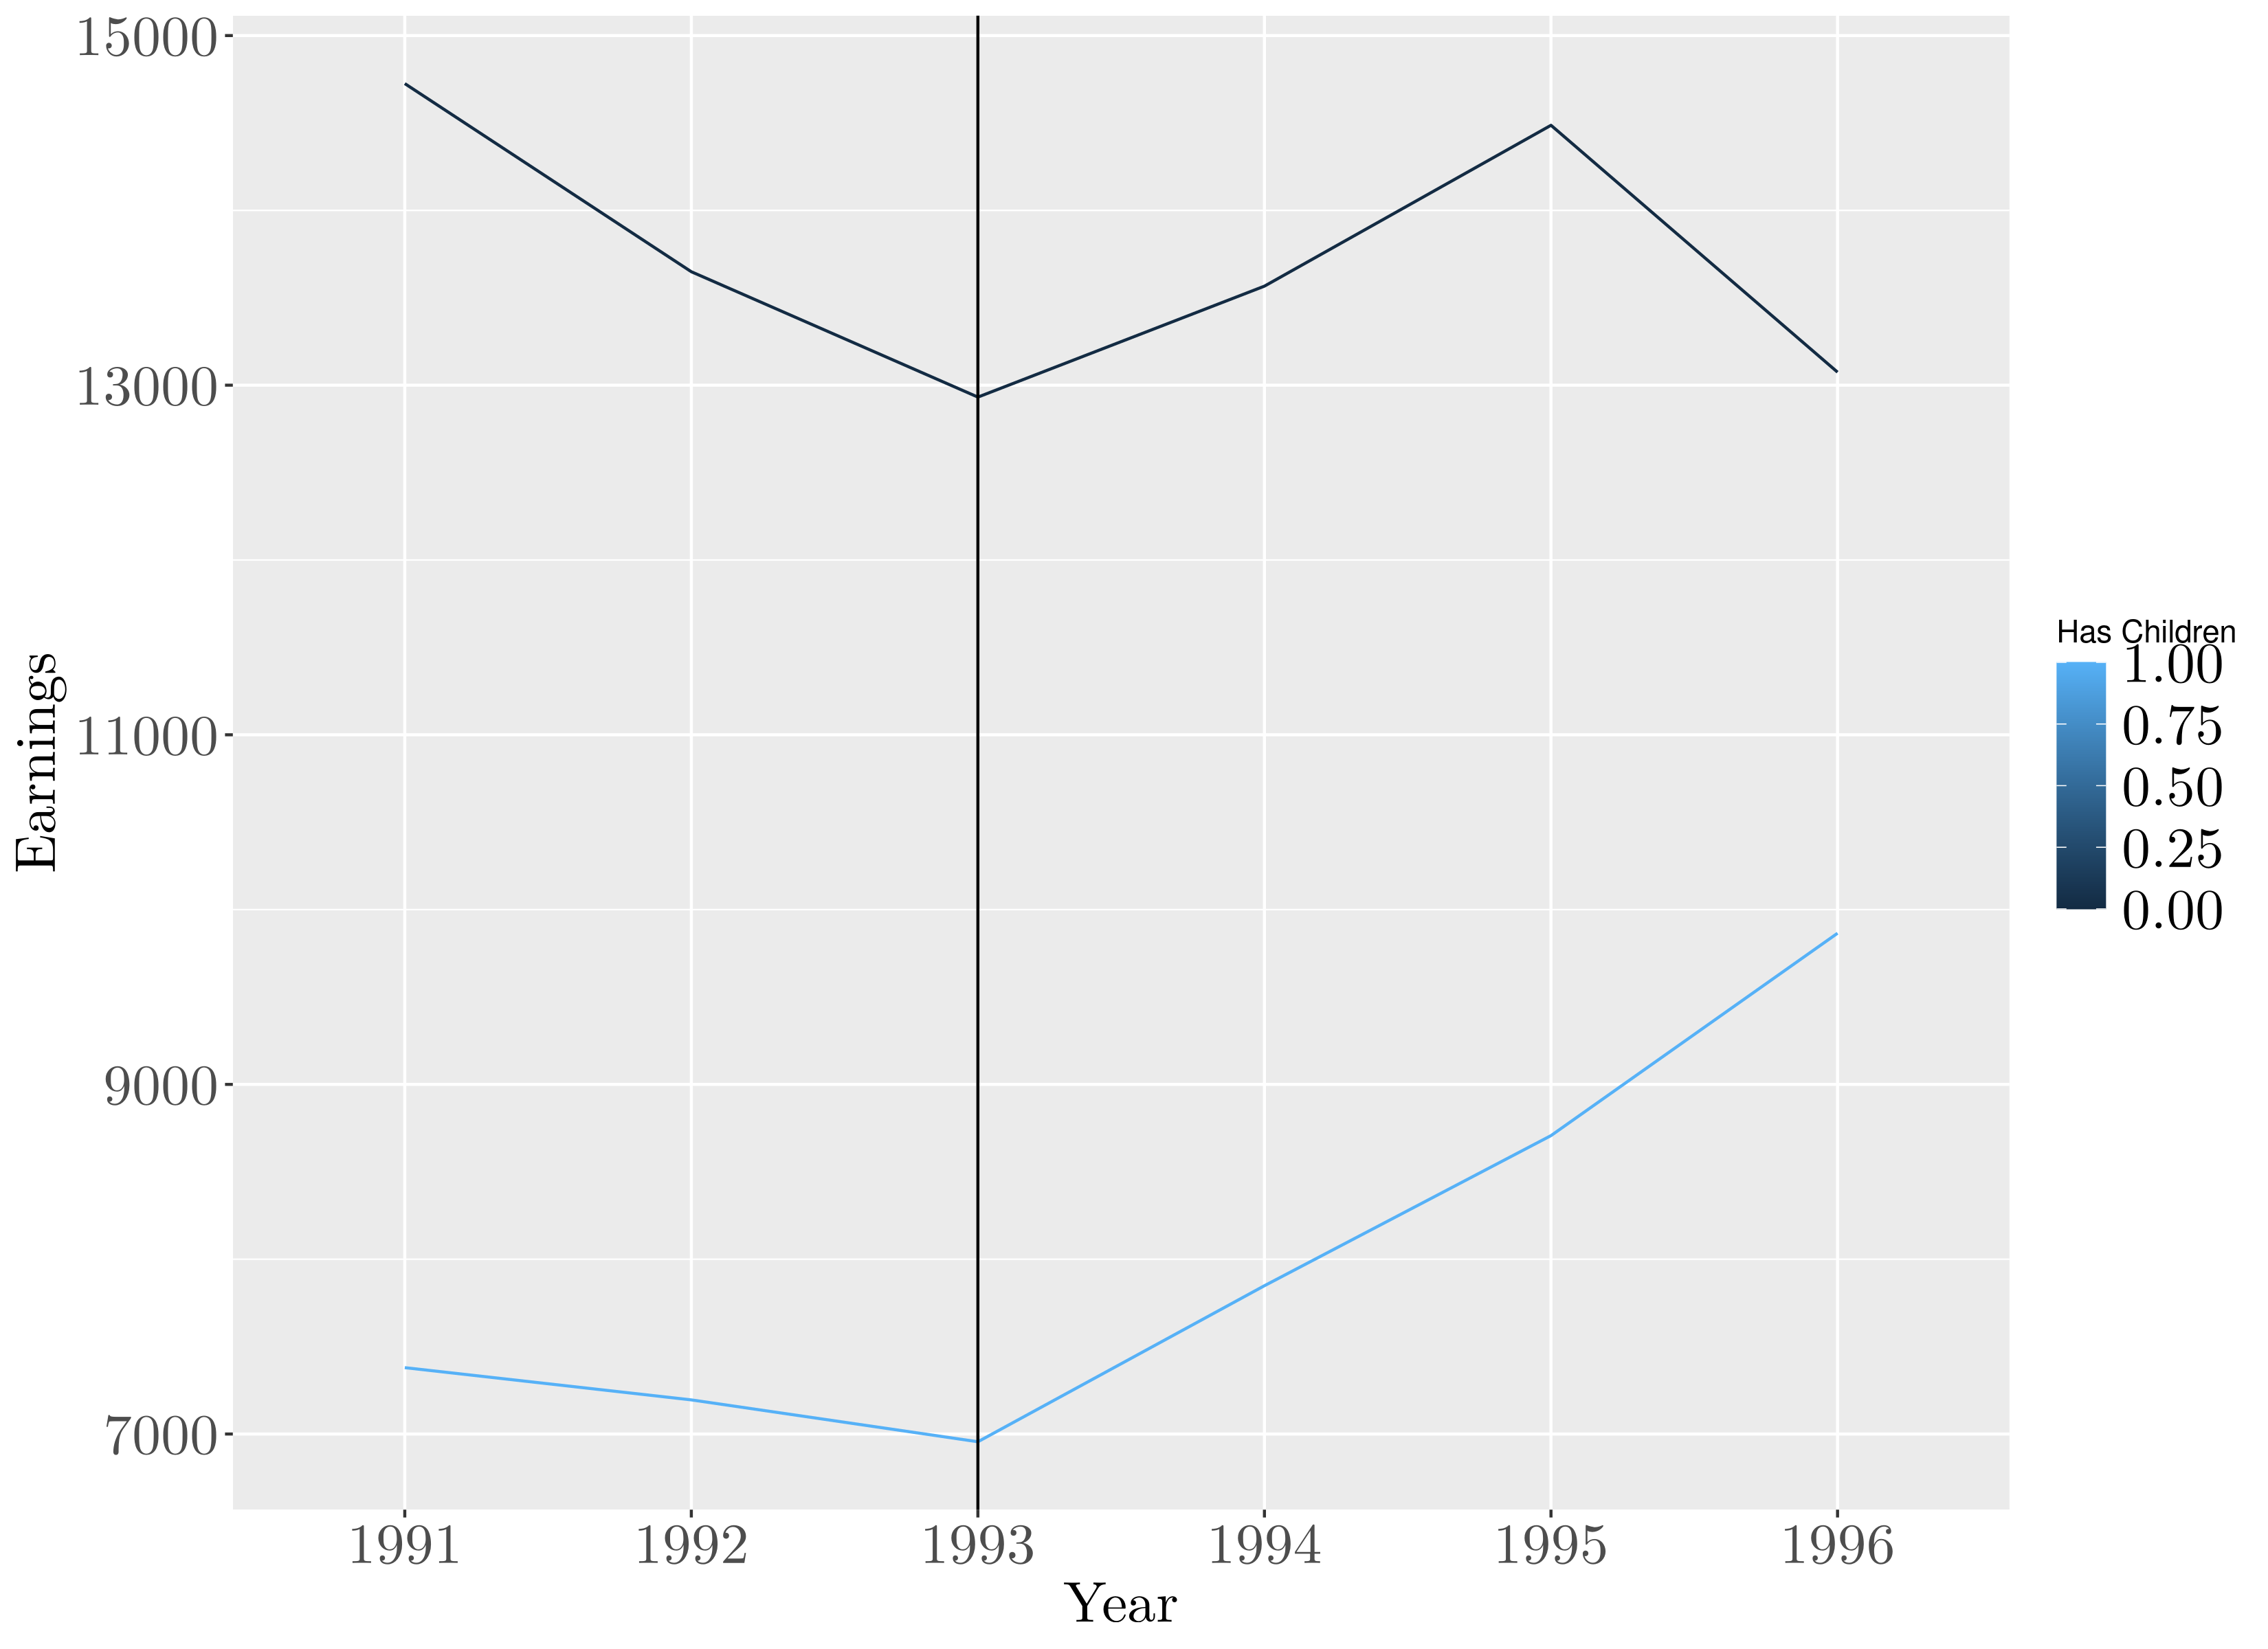
\includegraphics[width=.95\linewidth]{"/home/angelo/Documents/Uni/Courses/Advanced Statistics and programming/Assignments/assignment2/Graphics/task2_earn_did.png"} 
   \caption{Annual Earnings by Females with(out) Children}
   \label{fig:Ng2}
\end{subfigure}

\begin{subfigure}[b]{0.48\textwidth}
    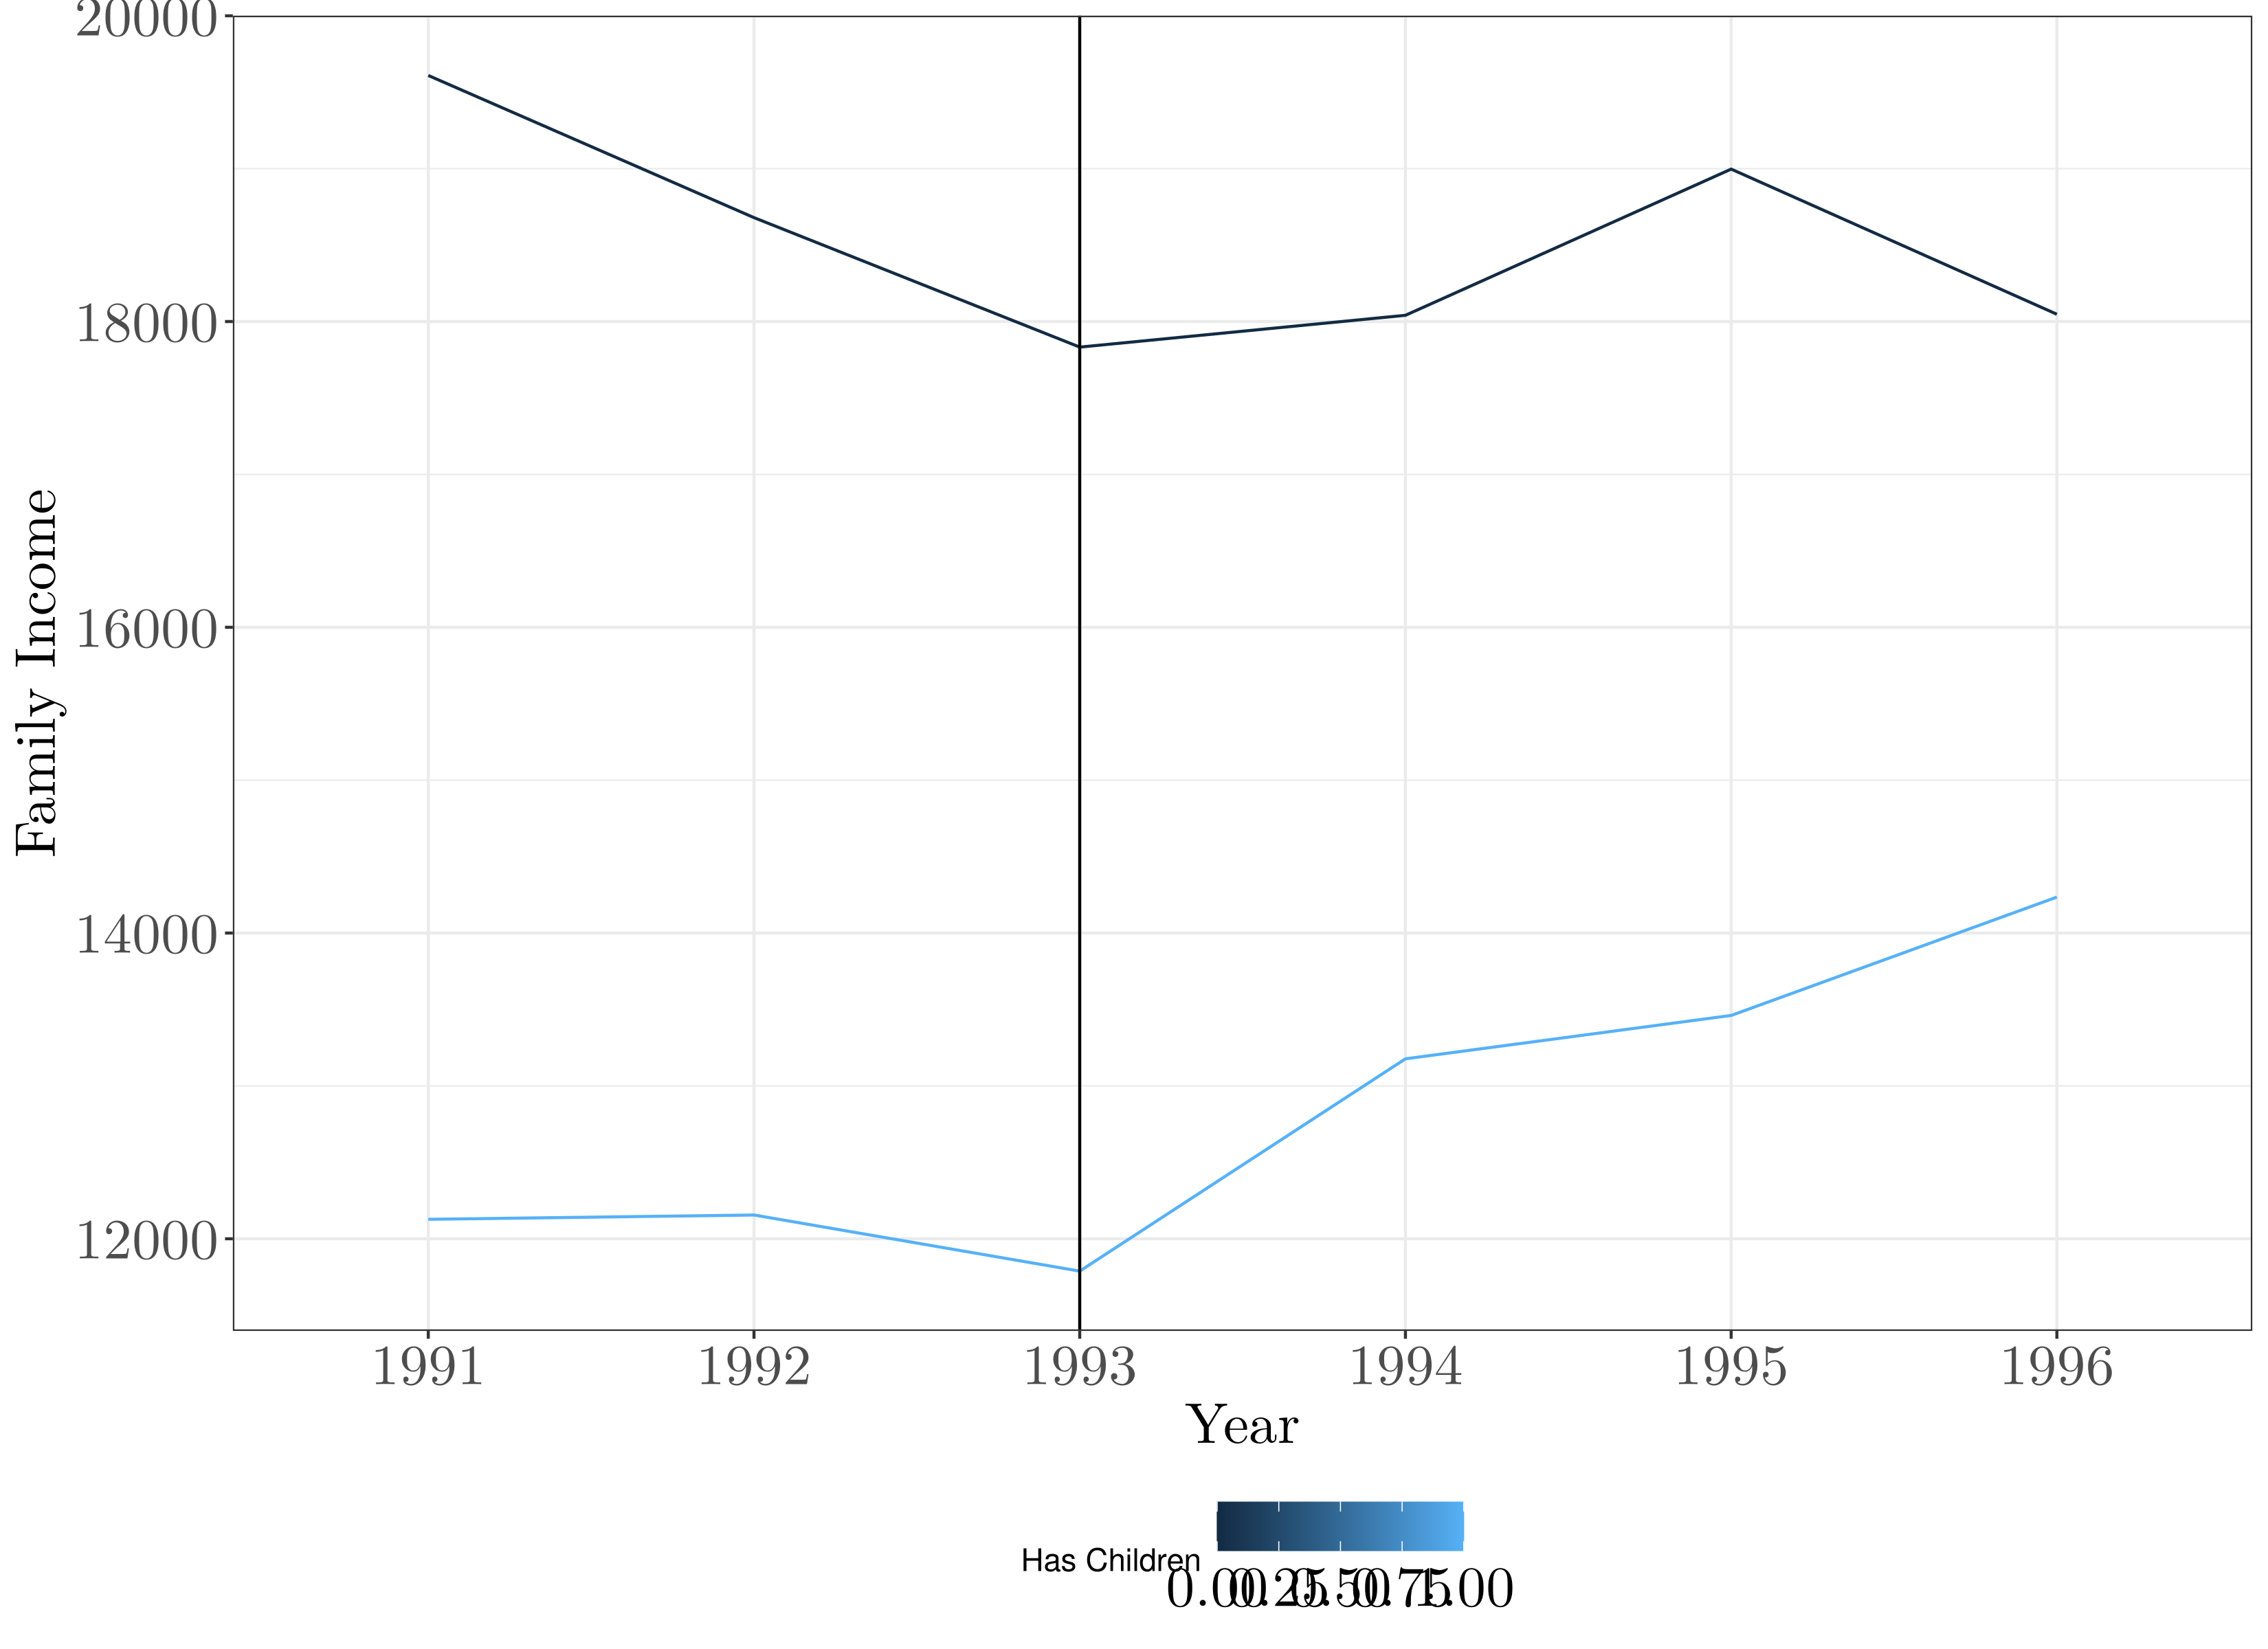
\includegraphics[width=.95\linewidth]{"/home/angelo/Documents/Uni/Courses/Advanced Statistics and programming/Assignments/assignment2/Graphics/task2_finc_did.png"} 
   \caption{Family Earnings Earnings by Females with(out) Children}
   \label{fig:Ng2}
\end{subfigure}

\begin{subfigure}[b]{0.48\textwidth}
    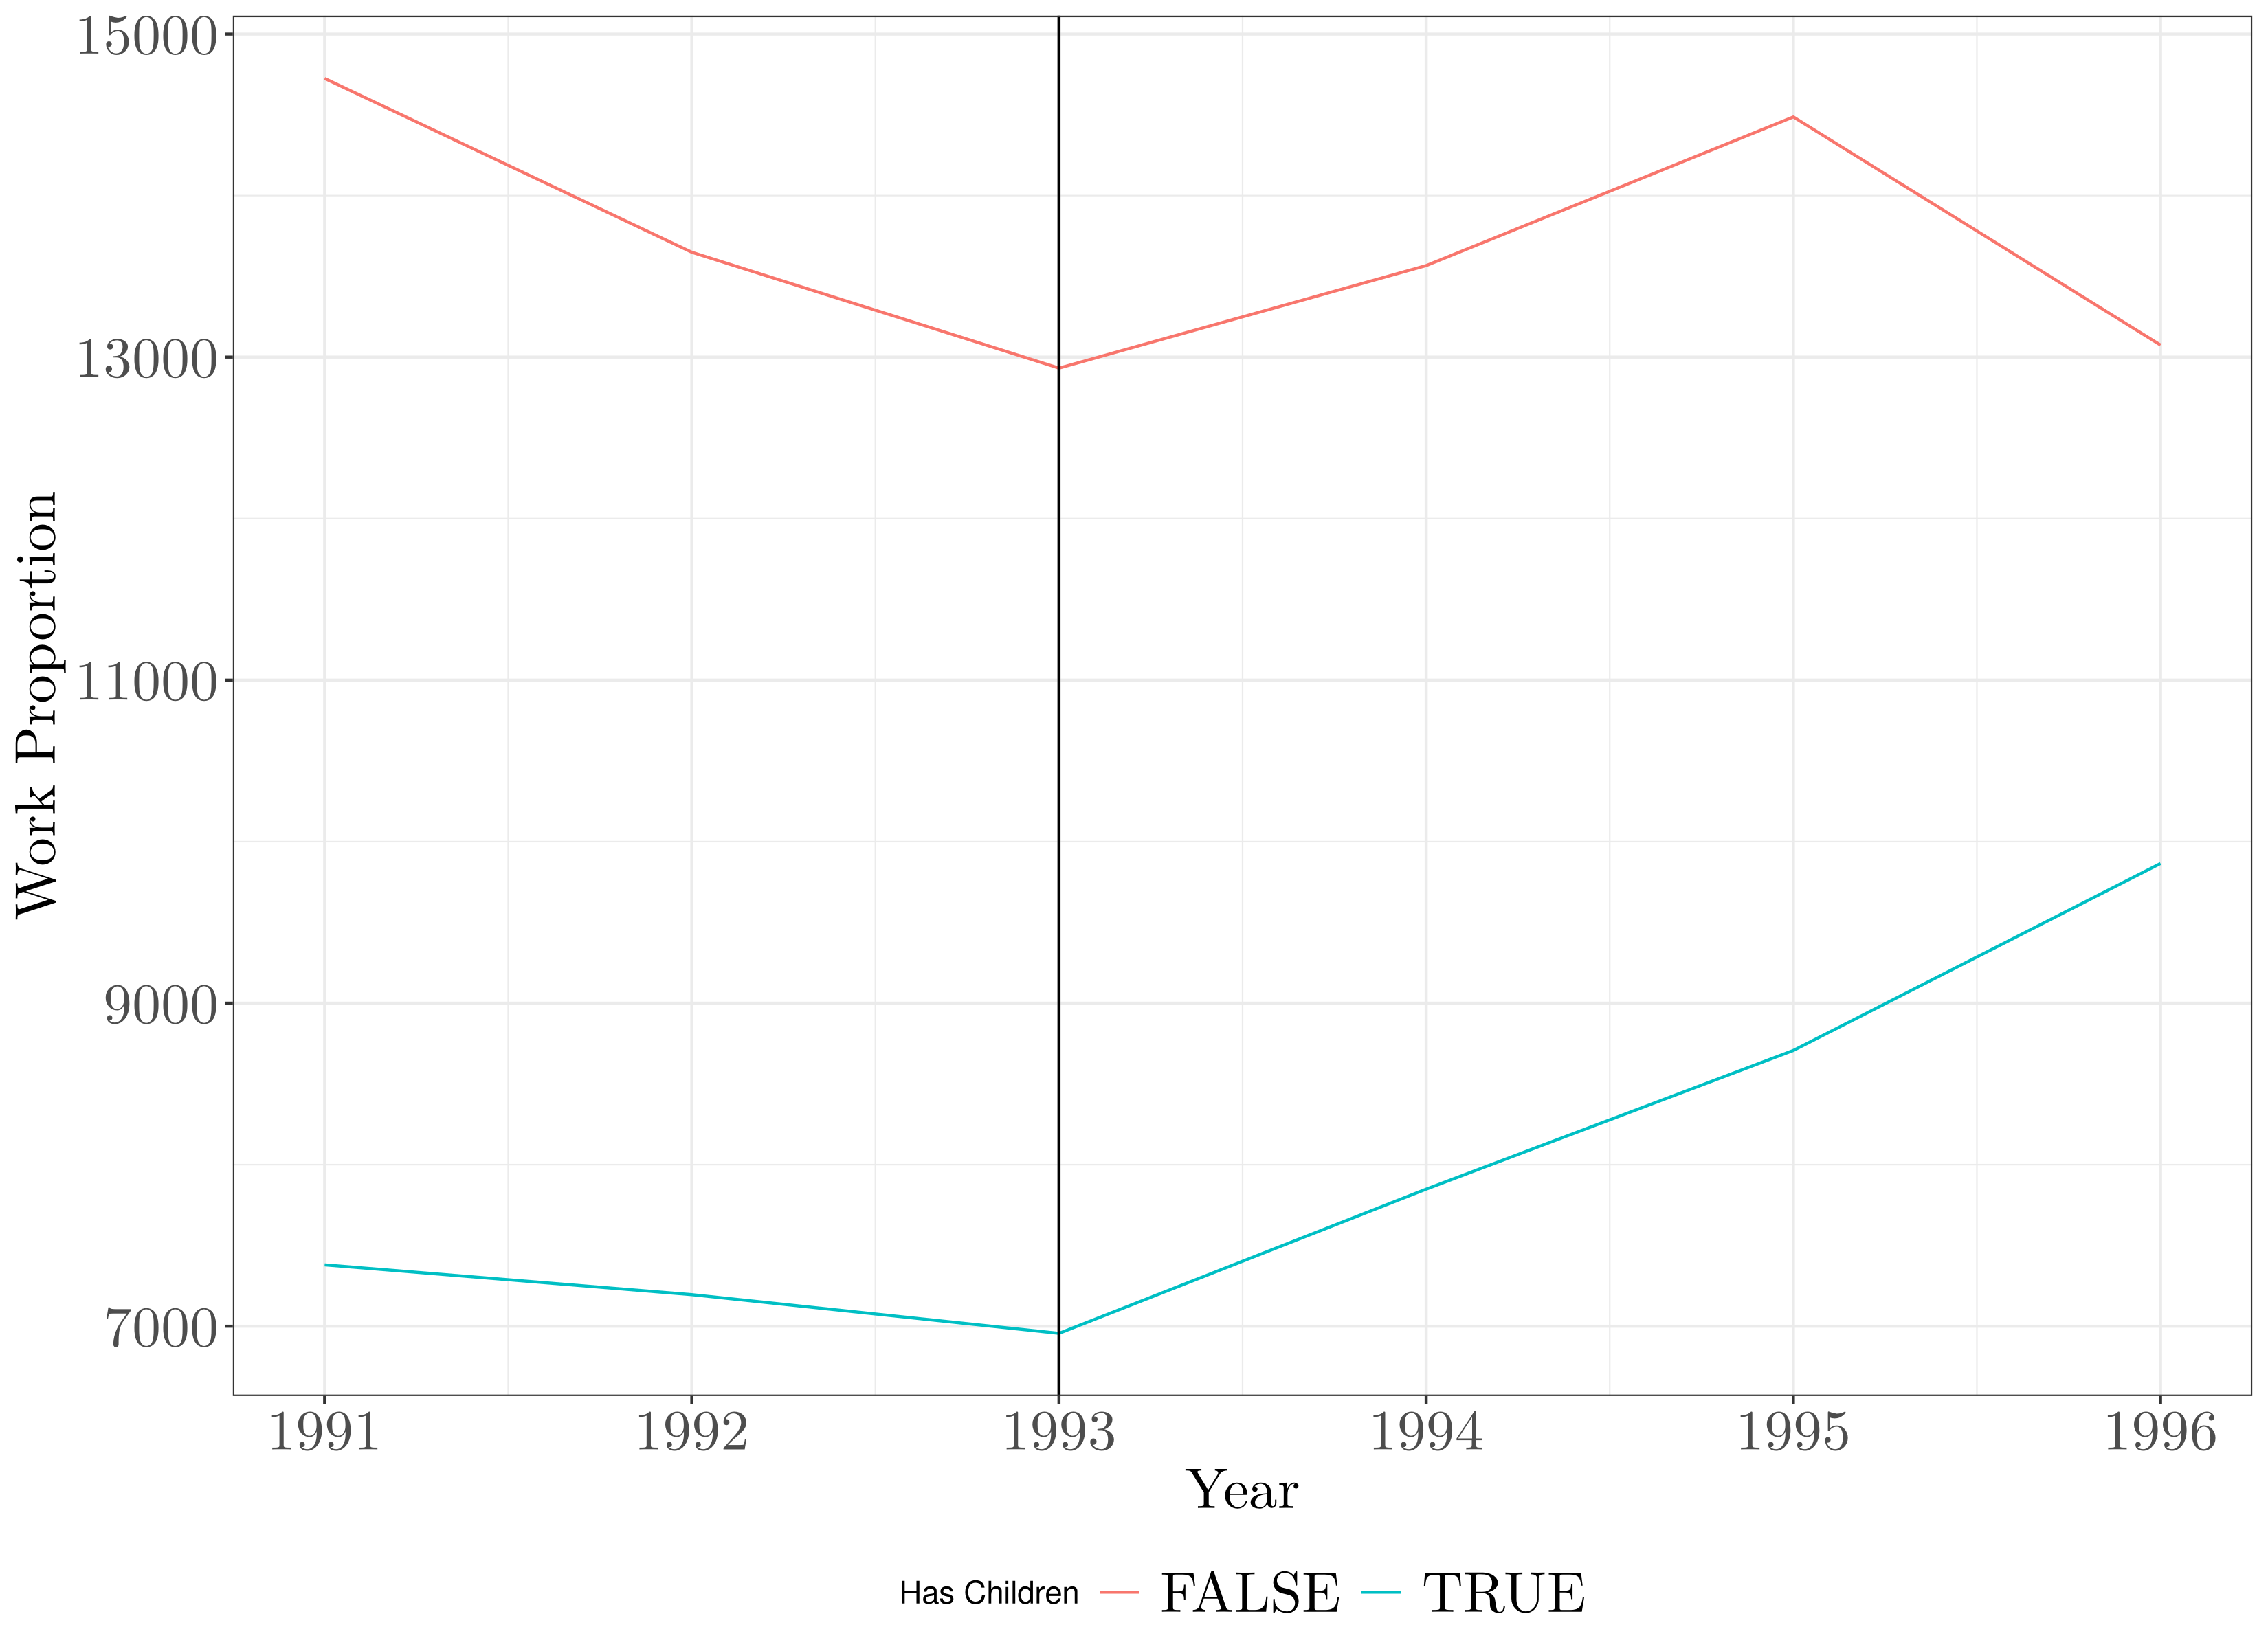
\includegraphics[width=.95\linewidth]{"/home/angelo/Documents/Uni/Courses/Advanced Statistics and programming/Assignments/assignment2/Graphics/task2_work_did.png"}  
   \caption{Work Participation by Females with(out) Children}
   \label{fig:Ng2}
\end{subfigure}
\captionsetup{justification=centering}
\caption{Pre-Post Intervention of EICT Credit for Women with(out) Children}
\end{wrapfigure}


Figure 1 displays the outcomes for both treatment and control group for earnings (earn), family income (finc), and work-participation indicator (work) over the period form 1991 to 1996. THe treatment in this case is defined as a binary state of females with children (one or many) (D = 1) and females without children (D = 0). The tax credit (EITC) is assumed to be introduced on the 1st of January 1993.
\indent Figure 1 a) displays the development of earnings and the introduction of the EITC is marked by the vertical line (as in the other graphics). Females without children earned considerably more on average than females with children (pre-period $mean$ = 7290.38) during the pre-period, starting out at slightly less than \$14800 and dropping to \$13000 at its lowest, with and average pre-intervention earnings of \$14203.90. Overall, both groups displayed a downward trend before 1993. After 1993, the supposed introduction of the EITC, both groups experienced an increase in earnings; However, the childless group did not display a continuous increase in earnings (post-period $mean$  = 13507.90) when compared to females with children (post-period $mean$  = 8277.20). This might suggest that the introduction of the  EITC is associated to the average earnings of women with children but not for women without children.
\indent Figure 1 b) shows the same features as the plot before but the outcome is now Family Income (numbers discussed in exercise 3 and 4). Overall, the general trend is similar for both groups as in Figure 1 a); it may be noted that the trend for females with child is less pronounced than in a). Nonetheless, the conclusion is the same as in a): During the pre-period, childless women earned more, but decreased stronger than women with children, while the post treatment movement is not continuous (dropping to pre treatment levels) for childless women when compared to women with children, which experience continuous growth on average.
\indent Figure 1 c) displays work-participation of females with and without children.Again, childless women start out higher at around 54\% work-participation vs 46\% work-participation for women with children. Moreover, the trends are somewhat comparable to the two preceding graphics, as females with children display an increase to 50.3\% (and then a slight drop in the following year), while childless women tend to decrease: As such, women with children again experience an average net gain in work participation during the post period, while childless women drop below pre-treatment levels. 


\subsection{Task 3: Summary Statistics for data}

The data-set is not balanced and we cannot assure that it is fixed. Nonetheless, for the purpose of this exercise, it is assumed that it is balanced and fixed. The data contains yearly records from 1991 to 1996; the reported values per variable are thus averages over all six years. Pre period is 1991 to 1992 and post treatment is 1993 to 1996. A total of 13746 records were made, split by year into 2610, 2449, 2342, 2255, and 2085 observations respectively. Of the total 13746 observations, 7819 have one or more children, and 5927 have no children.\footnote{additional summary statistics can be found for women with and without children in Appendix 4.1}. Of the relevant outcome variables (earnings, family income, work participation), the average family income was \$15255.32 ($std$ = 19444.24, $median$ = 9636.66). This large spread around the mean was partially addressed by Figure 1 a) displaying a large difference between women with and without children; this suggests a strong heterogeneity in the data wrt. to the outcomes. Additionally, as was to be expected by the financial nature of family income, there is a severe positive skewness of 7.06. Earnings displays a similar pattern as family income ($mean$ = 10432.48, $std$ = 18200.76, $median$ = 3332.18 $skew$ = 6.766), which is supported by Figure 1 b). As expected, earnings and family income correlate strongly with a Pearson correlation coefficient of .93 ($p$ $<$ 0.001); thus, earnings and family income are assumed to behave similarly as outcome variables. Finally, work participation shows that 51.3\% of records over all six years are in employment (std. and median have no meaning here as it is a binary variable). Considering possible covariates, the average years in education is 8.8 ($std$ = 2.636), with 11 years in the median. On average, per year, one women had 1.19 children ($std$ = 1.382, $median$ = 1), with 56.9\% of respondents having one child or more (N = 7819). Of the respondents 60\% were people of colour. Unemployment rate by state was on average 6.76\% ($std$ = 1.462, $median$ = 7.7) and unearned income at \$4823 ($std$ = 7123, $median$ = 6864).

\subsection{Task 4: Diff in Diff Matrix}


Table 2 reports the pre-post intervention averages for the two groups - Women with children and women without children - for earnings, family income, and work participation proportion; concluding in the DiD effect. Congruent with Figure 1 a) childless women have on average higher earnings in both pre- and post period than women with children (childless women diff mean diff pre-post: -696.00; women with children mean diff pre-post: 986.81). However, only women with children show a positive average gain over the post intervention period of \$986.81 (when compared to the average over the pre treatment period), while childless women even drop in earnings in the post period. Using formula (1-2) this results in a $naive$ DiD effect of \$1682.81 for women with children; which is simply the 1) difference within each group of pre and post intervention period and then 2) the difference between the groups. Again, a similar observation can be made for family income which displays a DiD of \$1911.04 (I am not repeating the numbers again). Finally, work participation also followed the trend observed in Figure 1 c), suggesting a DiD effect of 0.04 (or 4\% point gain ov women with children over childless women). Please note that these are just pre-post averages of the groups, complementing the descriptive statistics from part 2-3.


% Table created by stargazer v.5.2.3 by Marek Hlavac, Social Policy Institute. E-mail: marek.hlavac at gmail.com
% Date and time: Fri, Sep 23, 2022 - 21:38:43
% Requires LaTeX packages: dcolumn 
\begin{table}[!htbp] 
\begin{adjustwidth}{-0cm}{-0cm}
\begin{threeparttable}
\small
\captionsetup{font=small, justification=raggedright,singlelinecheck=false}
  \caption{Diff-in-Diff Matrix} 
  \label{} 
\begin{tabular}{@{\extracolsep{8pt}}lccccccc} 
\\[-5.8ex]\hline 
\hline \\[-1.8ex]
\multicolumn{2}{c}{}  & \multicolumn{2}{c}{Earning}  & \multicolumn{2}{c}{Family Income} & \multicolumn{2}{c}{Work Participation} \\ 
\multicolumn{1}{c}{} & \multicolumn{1}{c}{dperiod} & \multicolumn{1}{c}{Childless} & \multicolumn{1}{c}{Children} & \multicolumn{1}{c}{Childless} & \multicolumn{1}{c}{Children} & \multicolumn{1}{c}{Childless} & \multicolumn{1}{c}{Children} \\ 
\hline \\[-1.8ex] 
\multicolumn{1}{c}{Before} & 1 & 14,203.900 & 7,290.380 & 19,159.190 & 12,140.900 & 0.580 & 0.450 \\ 
\multicolumn{1}{c}{After} & 2 & 13,507.900 & 8,277.200 & 18,218.950 & 13,111.690 & 0.570 & 0.480 \\ 
\multicolumn{1}{c}{Difference} &  & -696.000 & 986.810 & -940.240 & 970.800 & -0.010 & 0.030 \\ 
\hline \\[-3.6ex] 
\end{tabular} 
\begin{tablenotes}[para,flushleft]
      \small
      \item\textit{Notes:} N = 5927 Childless; N = 7819 Has one or more Children.
    \end{tablenotes}
\end{threeparttable}
\end{adjustwidth}
\end{table}


\subsection{Task 5: Analyze the DiD regression}




\paragraph{No model without theory} Considering possible covariates, earnings, workparticipation, and family income all tend to vary with age (inverted u). Moreover, higher unemployment implies more labour supply and suppression of wages, family income and (obviously) work participation. Furthermore, higher education positively correlates with earnings, family income, and workparticipation. Finally, the US is known for racial tensions; people of colour tend to show lower incomes and lower work pariticpation in general (Morgan \& Winship, 2015). 



\paragraph{Results} For brevity reasons, Table 3 contains models for all three outcome variables, with the first model per outcome (1, 4, 7) containing a baseline model with only covariates. Models 2, 5, 8 contain only the DiD effects, and Models 3, 6, 9 contain the full model respectively. 

\indent Considerig earnings, the covariate model (1) shows only that nonwhite (indicator variable) ($\hat{\beta}$ = -2037.990, $p$ $<$ 0.001) and age ($\hat{\beta}$ = 96.038, $p$ $<$ 0.01) are significant. Overall, this model explains 0.6\% of the variation in earnings. Proceeding to only the DiD effect (model 2), as expected, women with children earn on average \$8596.33 ($p$ $<$ 0.01) less than childess women.\footnote{Note: the period indicator is not really relevant in such an exercise as compares the total trend change for two converging groups $y$} Subsequently, the value from Table 2 for the DiD effect is statistically significant at conventional levels, suggesting that women with children gain a \$1682.81 ($p$ $<$ 0.01) in the post treatment/intervention period (compared to pre period) (1993 $<$) when compared to childless women; overall explaining 2.6\% of the total variation in earnings. This effect is important to be examined more closely: As implied in task 4, while childless women on average earn \$ 8596.33 more than women with children, childless women (see Table 2) drop by \$696 when comparing the before and after period, while women with children increased. These two effects cancel each other out out, most likely leading to the insignificant period coefficient. Moreover, this suggests that the comparison groups (women with vs women without children) are not comparable; as such we will not be able to discern causality from this exercise. Finally, model (3) considers the full model. Focusing on the DiD effect after including covariates, we see a slight increase in the coefficient ($\hat{\beta}$ = 1722.360, $p$ $<$ 0.01) with stable standard errors; suggesting that women with children in the post period earn \$1722.36 more than childless women. However, the inclusion of the covariates does not suggest a considarable change in the direction of the outcome. 
\indent Moving to family income as an outcome, a similar insights can be drawn. However, now all covariates are significant - model explaining 1.2\% of the variation in family income. Again, the DiD effect alone in model (5) is significant ($\hat{\beta}$ = 1911.04, $p$ $<$ 0.01); suggesting again that women with childrens' familiy income increases by \$1911.04 after the intervention (when compared to the pre-period) when compared to childess women. Additionally, women with children, again, have a lower family income of \$-8929.33 ($p$ $<$ 0.01). This model explains 2.2\% of the total variation in family income. The inclusion of covariates does not change this insight dramitically; womens' with children family income still improve significantly by \$2006.06 during the post period when compared to childess women and its coefficeint also increases, but the insight is the same as before ($p$ $<$ 0.01). 
\indent Finally, considering work participation; the covariates in model (7) are all significant at the conventional level in predicting work participation, explaining 1.9\% of total variation in this outcome. As observed during task 1 through 4, work participation rises for women with children during the post intervention period (model 8) ($\hat{\beta}$ = 0.031, $p$ $<$ 0.1); however, the effect is only marinally significant. As was to be expected, women with children show a significantly lower work participation ($\hat{\beta}$ = -0.159, $p$ $<$ 0.01) when compared to childless women (15.9\$ less). When combining covariates and the base model in model (9), the overall trend is the same as in the aforementioned models. The coefficient for the DiD effect rises to 0.033 ($p$ $<$ 0.1), but is still only marginally significant.
Thus, overall, the inclusion of the covaraites does increase the coefficints of all three DiD effects, but only marginally. This means that the overall effect, or direction of the coefficicients was not changed drastically. Moreover, the inclusion of the covariates shows that the standard errors are stable across all models, suggesting no probelm with multicollinearity. 
\paragraph{Robustness Tests} Overall, due to the standard errrors between the models for each outcome variable respectively staying stable, this suggests that there is generally less necessity to include robust standard errors. Running the Breusch-Pagan test on all models in Table 3 - only model (1) and model (4) (both covariate-only models) fail to reject the null hypothesis of heteroscedasitc residuals. Finally, Table 11 in the appendix reports robust standard errors (white) and clustered by state. Overall, the standard errors are stable across models, which suggests, that there is little need to use robust standard errors; inference is not changed.\footnote{Stability in coefficients also implies no multicollinearity; additionally, standardized coefficeints are not of use here becasue we are interested in the DiD effect.} 


\begin{landscape}
% Table created by stargazer v.5.2.3 by Marek Hlavac, Social Policy Institute. E-mail: marek.hlavac at gmail.com
% Date and time: Wed, Sep 28, 2022 - 18:35:54
\begin{table}[!htbp] \centering 
\begin{adjustwidth}{1.25cm}{-0cm}
\begin{threeparttable}
\small
\captionsetup{font=small, justification=raggedright,singlelinecheck=false}
\caption{\textsc{Non-Robust Regression Results Part 3}}
\centering 
  \label{}
\small 
\begin{tabular}{@{\extracolsep{-2pt}}lccccccccc} 
\\[-5.8ex]\hline 
\hline \\[-1.8ex] 
 & \multicolumn{9}{c}{\textit{Dependent variable:}} \\ 
\cline{2-10} 
\\[-1.8ex] & \multicolumn{3}{c}{earn} & \multicolumn{3}{c}{finc} & \multicolumn{3}{c}{work} \\ 
\\[-1.8ex] & (1) & (2) & (3) & (4) & (5) & (6) & (7) & (8) & (9)\\ 
\hline \\[-1.8ex] 
 Constant & 7,977.343$^{***}$ & 14,899.900$^{***}$ & 12,958.640$^{***}$ & 11,872.150$^{***}$ & 20,099.430$^{***}$ & 16,218.430$^{***}$ & 0.414$^{***}$ & 0.582$^{***}$ & 0.532$^{***}$ \\ 
  & (1,159.632) & (828.375) & (1,550.012) & (1,234.711) & (886.522) & (1,655.347) & (0.032) & (0.023) & (0.043) \\ 
  & & & & & & & & & \\ 
 Age & 96.038$^{***}$ &  & 22.555 & 144.373$^{***}$ &  & 78.717$^{***}$ & 0.003$^{***}$ &  & 0.002$^{***}$ \\ 
  & (15.489) &  & (15.922) & (16.492) &  & (17.004) & (0.0004) &  & (0.0004) \\ 
  & & & & & & & & & \\ 
 Unemp. Rate & 33.433 &  & 133.948 & 256.102$^{**}$ &  & 372.861$^{***}$ & $-$0.018$^{***}$ &  & $-$0.018$^{***}$ \\ 
  & (108.495) &  & (114.614) & (115.519) &  & (122.403) & (0.003) &  & (0.003) \\ 
  & & & & & & & & & \\ 
 Education (y) & 8.153 &  & 66.337 & $-$177.633$^{***}$ &  & $-$125.305$^{**}$ & 0.016$^{***}$ &  & 0.017$^{***}$ \\ 
  & (60.120) &  & (59.579) & (64.013) &  & (63.628) & (0.002) &  & (0.002) \\ 
  & & & & & & & & & \\ 
 Race & $-$2,037.990$^{***}$ &  & $-$1,255.622$^{***}$ & $-$3,109.127$^{***}$ &  & $-$2,438.387$^{***}$ & $-$0.058$^{***}$ &  & $-$0.043$^{***}$ \\ 
  & (323.611) &  & (326.237) & (344.563) &  & (348.408) & (0.009) &  & (0.009) \\ 
  & & & & & & & & & \\ 
 Has Child &  & $-$8,596.327$^{***}$ & $-$8,394.973$^{***}$ &  & $-$8,929.330$^{***}$ & $-$8,269.567$^{***}$ &  & $-$0.159$^{***}$ & $-$0.150$^{***}$ \\ 
  &  & (1,093.444) & (1,096.506) &  & (1,170.197) & (1,171.022) &  & (0.030) & (0.030) \\ 
  & & & & & & & & & \\ 
 dperiod &  & $-$695.997 & $-$536.491 &  & $-$940.239$^{*}$ & $-$515.553 &  & $-$0.005 & $-$0.024$^{*}$ \\ 
  &  & (485.413) & (500.046) &  & (519.486) & (534.028) &  & (0.013) & (0.014) \\ 
  & & & & & & & & & \\ 
 has\_children1:dperiod &  & 1,682.810$^{***}$ & 1,722.360$^{***}$ &  & 1,911.035$^{***}$ & 2,006.060$^{***}$ &  & 0.031$^{*}$ & 0.033$^{*}$ \\ 
  &  & (642.099) & (641.893) &  & (687.171) & (685.515) &  & (0.018) & (0.018) \\ 
  & & & & & & & & & \\ 
\hline \\[-1.8ex] 
Observations & 13,746 & 13,746 & 13,746 & 13,746 & 13,746 & 13,746 & 13,746 & 13,746 & 13,746 \\ 
R$^{2}$ & 0.006 & 0.026 & 0.027 & 0.012 & 0.022 & 0.028 & 0.019 & 0.012 & 0.027 \\ 
Adjusted R$^{2}$ & 0.006 & 0.026 & 0.027 & 0.012 & 0.022 & 0.027 & 0.018 & 0.012 & 0.026 \\ 
Residual Std. Error & 18,150.240  & 17,965.670  & 17,956.450 & 19,325.370 & 19,226.750  & 19,176.730  & 0.495  & 0.497  & 0.493  \\ 
F Statistic & 20.153$^{***}$  & 121.691$^{***}$  & 54.794$^{***}$ & 43.406$^{***}$  & 105.245$^{***}$  & 56.166$^{***}$ & 65.588$^{***}$  & 54.906$^{***}$  & 54.374$^{***}$  \\
\hline 
\hline \\[-3.5ex] 
\end{tabular} 
\begin{tablenotes}[para,flushleft]
      \small
      \item\textit{Note:} N = 13746. Non Robust Standard Errors applied. "White" is reference category for "non-White" categorical variable. First model of each outcome ony covariates; second model only DiD effect with causal varaibles; thrid model complete. *** p$<$0.01, ** p$<$0.05, * p$<$0.1.
    \end{tablenotes}
\end{threeparttable}
\end{adjustwidth}
%
\end{table}

\end{landscape}


\subsection{Task 6: Subset analysis}

\subsubsection{Women with Children compared based on high \& low education levels}
Please note: after sub-setting the data per sub-task, interaction effects were used in order to maintain statistical power of the model (the interpretation is the same).
For brevity reasons, the covariate only models are left out (intuition does not change when compared to table 3). Considering now only women with children: the "difference in groups" as women with high vs low education, table 4 reports a baseline and a complete model per outcome. The comparison group is low education women with children.
Considering earnings, (model 1 \& 2), the DiD coefficient is interpreted as follows: during the post intervention period (compared to the pre-intervention period), high educated women gain 951.50\$ on average ($p$ $=$ 0.216) compared to low educated women; which however is not significant. This is broadly maintained when only considering the base model ($\hat{\beta}$ = 871.46, $p$ $<$ 0.26). A similar observation can be made for work participation, which is in both cases, the base model (5) and with covaraites (6), displaying an insignificant decrease in work participation for highly educated women (compared to low educated women) in the post intervention period when compared to the per-period ($\hat{\beta}$ = -0.019, $p$ $=$ 0.462). Finally, family income observed a marginally significant increase of \$1345.12 at the 9.4\% percent level for highly educated women during the post period compared to low educated women, while the base model is insignificant at the 15.2\% level for the DiD effect of education and intervention period. 







% Table created by stargazer v.5.2.3 by Marek Hlavac, Social Policy Institute. E-mail: marek.hlavac at gmail.com
% Date and time: Wed, Sep 14, 2022 - 15:53:27
\begin{table}[!htbp] \centering 
\begin{adjustwidth}{0.cm}{-0cm}
\begin{threeparttable}
\small
\captionsetup{font=small, justification=raggedright,singlelinecheck=false}
\caption{\textsc{Subsection Analysis Single Women with Children for alternating low/ high education levels}}
\centering 
  \label{}
\small 
\begin{tabular}{@{\extracolsep{-1pt}}lcccccc} 
\\[-5.8ex]\hline 
\hline \\[-1.8ex] 
 & \multicolumn{6}{c}{\textit{Dependent variable:}} \\ 
\cline{2-7} 
\\[-1.8ex] & \multicolumn{2}{c}{earn} & \multicolumn{2}{c}{finc} & \multicolumn{2}{c}{work} \\ 
\\[-1.8ex] & (1) & (2) & (3) & (4) & (5) & (6)\\ 
\hline \\[-1.8ex] 
 Constant & 8,743.660$^{***}$ & 4,625.713$^{***}$ & 13,755.130$^{***}$ & 4,175.858$^{**}$ & 0.422$^{***}$ & 0.527$^{***}$ \\ 
  & (1,108.213) & (1,691.462) & (1,166.890) & (1,768.019) & (0.037) & (0.057) \\ 
  edu\_lvl & $-$3,427.529$^{***}$ & $-$3,177.416$^{**}$ & $-$3,629.042$^{***}$ & $-$3,079.124$^{**}$ & 0.002 & 0.006 \\ 
  & (1,311.705) & (1,306.105) & (1,381.156) & (1,365.220) & (0.044) & (0.044) \\ 
  dperiod & 370.227 & 416.590 & 142.756 & 453.880 & 0.011 & $-$0.009 \\ 
  & (653.474) & (658.753) & (688.073) & (688.568) & (0.022) & (0.022) \\ 
  age &  & 174.206$^{***}$ &  & 272.964$^{***}$ &  & 0.004$^{***}$ \\ 
  &  & (20.082) &  & (20.991) &  & (0.001) \\ 
  urate &  & $-$34.414 &  & 261.583$^{**}$ &  & $-$0.025$^{***}$ \\ 
  &  & (127.034) &  & (132.784) &  & (0.004) \\ 
  nonwhite1 &  & $-$2,547.489$^{***}$ &  & $-$3,380.644$^{***}$ &  & $-$0.061$^{***}$ \\ 
  &  & (368.752) &  & (385.442) &  & (0.012) \\ 
  edu\_lvl:dperiod & 871.461 & 951.502 & 1,166.212 & 1,345.136$^{*}$ & 0.021 & 0.019 \\ 
  & (773.065) & (767.593) & (813.996) & (802.335) & (0.026) & (0.026) \\ 
 \hline \\[-1.8ex] 
Observations & 7,819 & 7,819 & 7,819 & 7,819 & 7,819 & 7,819 \\ 
R$^{2}$ & 0.005 & 0.020 & 0.004 & 0.033 & 0.002 & 0.016 \\ 
Adjusted R$^{2}$ & 0.004 & 0.020 & 0.003 & 0.033 & 0.001 & 0.016 \\ 
Residual Std. Error & 14,923.420& 14,810.030 & 15,713.570 & 15,480.340  & 0.499  & 0.495 \\ 
F Statistic & 12.717$^{***}$  & 26.977$^{***}$ & 9.460$^{***}$ & 44.915$^{***}$  & 4.884$^{***}$  & 21.557$^{***}$  \\ 
\hline 
\hline \\[-3.5ex] 
\end{tabular} 
\begin{tablenotes}[para,flushleft]
      \small
      \item\textit{Note:} N = 7819 Single Women have Children. N = 5593 high education (years of eduction $>$= 9 years); N = 2226 low education (years of eduction $<$ 9 years); Non Robust Standard Errors applied. "White" is reference category for "non-White" categorical variable. *** p$<$0.01, ** p$<$0.05, * p$<$0.1.
    \end{tablenotes}
\end{threeparttable}
\end{adjustwidth}
%
\end{table}

\subsubsection{Women with and without Children compared keeping education level (low) constant}

Considering now only low educated women; alternating again on whether a women has a child or not, the insights are to be found in Table 5. 
The subsection analysis shows that the post intervention period earnings for low educated women with children decrease by \$413.45 when compared to women without children in the base model; however all insignificant ($p$ $=$ 0.730). This does not change for the complete model ($\hat{\beta}$ = -475.403, $p$ $<$ 0.691). Same can be observed for the outcome variables Family Income (main model: $\hat{\beta}$ = -179.637, $p$ $=$ 0.887) and work participation (main model: $\hat{\beta}$ = 0.012, $p$ $=$ 0.702). Thus, there is no statistical support that work participation rises by 1.2\% for women with children compared to childless women during the post intervention period and likewise for family income decreases.\footnote{this would have been very interesting; because if work would go up significantly while income drops, this would be crazy.}
Overall, the introduction of the tax credit does not seem to display a significant DiD across the different outcoems and subgroups.


% Table created by stargazer v.5.2.3 by Marek Hlavac, Social Policy Institute. E-mail: marek.hlavac at gmail.com
% Date and time: Wed, Sep 14, 2022 - 15:53:27
\begin{table}[!htbp] \centering 
\begin{adjustwidth}{0.cm}{-0cm}
\begin{threeparttable}
\small
\captionsetup{font=small, justification=raggedright,singlelinecheck=false}
\caption{\textsc{Subsection Analysis Single Women with/ without Children for constant (low) education levels}}
\centering 
  \label{}
\small 
\begin{tabular}{@{\extracolsep{3pt}}lcccccc} 
\\[-5.8ex]\hline 
\hline \\[-1.8ex] 
 & \multicolumn{6}{c}{\textit{Dependent variable:}} \\ 
\cline{2-7} 
\\[-1.8ex] & \multicolumn{2}{c}{earn} & \multicolumn{2}{c}{finc} & \multicolumn{2}{c}{work} \\ 
\\[-1.8ex] & (1) & (2) & (3) & (4) & (5) & (6)\\ 
\hline \\[-1.8ex] 
 Constant & 11,066.700$^{***}$ & 4,281.758 & 17,494.530$^{***}$ & 8,507.214$^{***}$ & 0.501$^{***}$ & 0.441$^{***}$ \\ 
  & (1,457.343) & (2,602.848) & (1,534.185) & (2,735.084) & (0.038) & (0.068) \\ 
  has\_children1 & $-$2,323.038 & $-$2,402.722 & $-$3,739.399$^{*}$ & $-$3,267.950 & $-$0.080 & $-$0.087 \\ 
  & (2,026.514) & (2,030.169) & (2,133.367) & (2,133.311) & (0.053) & (0.053) \\ 
  dperiod & 783.677 & 1,378.102 & 322.393 & 1,127.629 & $-$0.004 & $-$0.007 \\ 
  & (858.662) & (882.127) & (903.937) & (926.943) & (0.023) & (0.023) \\ 
  age &  & 29.868 &  & 83.479$^{***}$ &  & 0.001 \\ 
  &  & (29.856) &  & (31.373) &  & (0.001) \\ 
  urate &  & 651.163$^{***}$ &  & 845.832$^{***}$ &  & $-$0.002 \\ 
  &  & (216.731) &  & (227.742) &  & (0.006) \\ 
  nonwhite1 &  & 332.812 &  & $-$2,403.220$^{***}$ &  & 0.081$^{***}$ \\ 
  &  & (664.392) &  & (698.146) &  & (0.017) \\ 
  has\_children1:dperiod & $-$413.449 & $-$475.403 & $-$179.637 & $-$152.761 & 0.015 & 0.012 \\ 
  & (1,194.473) & (1,193.612) & (1,257.455) & (1,254.253) & (0.031) & (0.031) \\ 
 \hline \\[-1.8ex] 
Observations & 4,311 & 4,311 & 4,311 & 4,311 & 4,311 & 4,311 \\ 
R$^{2}$ & 0.006 & 0.009 & 0.010 & 0.016 & 0.003 & 0.008 \\ 
Adjusted R$^{2}$ & 0.006 & 0.008 & 0.009 & 0.015 & 0.002 & 0.007 \\ 
Residual Std. Error & 18,962.540 & 18,944.100 & 19,962.390  & 19,906.540  & 0.498  & 0.497 \\ 
F Statistic & 9.304$^{***}$ & 6.559$^{***}$  & 14.690$^{***}$ & 11.920$^{***}$ & 4.494$^{***}$ & 6.121$^{***}$  \\ 
\hline 
\hline \\[-3.5ex] 
\end{tabular} 
\begin{tablenotes}[para,flushleft]
      \small
      \item\textit{Note:} N = 4311 Single Women have Children (years of eduction $<$ 9 years). N = 2085 has no children; N = 2226 has children; Non Robust Standard Errors applied. "White" is reference category for "non-White" categorical variable. *** p$<$0.01, ** p$<$0.05, * p$<$0.1.
    \end{tablenotes}
\end{threeparttable}
\end{adjustwidth}
%
\end{table}

\section{Instrumental Variable approach}

\subsection{Task 1: Endogineity problems and correlation with u - A3}
When considering the problem of mean independence (A3), there can be multiple root causes to this issue; ommitted variable bias, sampling bias, attrition bais, simultaneous caulsailty bias. All of these issues introduce backdoor pathways, which bias the (eg. OLS) estimator severely (Morgan \& Winship, 2015). 
A prominent example in what way education effect on earnings could be biased is through an ommitted varaible. A classical example for this is general ability, which commonly determines not only the degree of success in education, but also future earnings. Through this, education would correlate with the disturbance term, violating A3. Thus, neglecting to include this confounder, will lead to a biased estimate of the effect of years of education on earnings.
A second example could be socioeconomic factors. Not only tend wealthier families to send their children to better schools, but also do such children participate more often in tertiary education; thereby impacting years of education. Contrarily, worse off families may require their children to drop out of school to contribute to the family income (considering that it is the 1950s this is not unlikely). Moreover, wealthy family tend to create more job opportunitities for their children through connections and inheritance etc.. Thus, socioeconomic status of the family not only impacts the duration (years) of education of their child, but also their later income. This is not only decribing omitted variable bias, but also (self) selection bias into another (higher ed) treatment group; another detrimental bias.

\subsection{Task 2: Summary statistics for this task}

Table 6 contains the descriptive statistics of the numeric variables. Overall 329,509 observations are in the data on people born between 1930 and 1939. The age range of study subjects ranges from 40 to 50, with a median age at 45 ($mean$ = 44.645, $std$ = 2.940). The average years of education was 12.77 ($std$ = 3.281, $median$ = 12). Finally, for interpretation purposes here, lnwage ($mean$ = 5.90, $std$ = 0.679, $median$ = 6.257) was re-scaled to wage, which displayed a strong positive skew of 26.39, mean of \$439.47 ($std$ = 364.941) and a median of \$521.85. The log scaled wage will be used during the analysis. 
Moreover, 86.3\% of respondents were married. SMSA indicates whether a study subject lives in rural or urban areas. Quarter of birth, the IV, distributes reasonably equally, with Q1 N = 81671, Q2 N = 80138, Q3 N = 86856, and Q4 N = 80844 - it is influential to when a study subject will start schooling; eg. suggesting that subjects from the fourth quarter generally obtain more years of study.  

% Table created by stargazer v.5.2.3 by Marek Hlavac, Social Policy Institute. E-mail: marek.hlavac at gmail.com
% Date and time: Sun, Sep 25, 2022 - 15:43:50
\begin{table}[!htbp] 
\begin{adjustwidth}{-0cm}{-0cm}
\begin{threeparttable}
\small
\captionsetup{font=small, justification=raggedright,singlelinecheck=false}
  \caption{Instrumental Vairable Approach Descriptive Statistics of Numeric Indepdenent and Dependent Varaible} 
  \label{} 
\begin{tabular}{@{\extracolsep{5pt}}lccccccc} 
\\[-5.8ex]\hline 
\hline \\[-1.8ex] 
Statistic & \multicolumn{1}{c}{Mean} & \multicolumn{1}{c}{St. Dev.} & \multicolumn{1}{c}{Min} & \multicolumn{1}{c}{Pctl(25)} & \multicolumn{1}{c}{Median} & \multicolumn{1}{c}{Pctl(75)} & \multicolumn{1}{c}{Max} \\ 
\hline \\[-1.8ex] 
Age & 44.645 & 2.940 & 40 & 42 & 45 & 47 & 50 \\ 
Education in Years & 12.770 & 3.281 & 0 & 12 & 12 & 15 & 20 \\ 
lnwage & 5.900 & 0.679 & $-$2.342 & 5.637 & 5.952 & 6.257 & 10.532 \\ 
Wage & 439.471 & 364.941 & 0.096 & 280.481 & 384.711 & 521.848 & 37,499.990 \\ 
Quarter of Birth & 2.506 & 1.112 & 1 & 2 & 3 & 3 & 4 \\ 
\hline \\
[-3.5ex] 
\end{tabular} 
\begin{tablenotes}[para,flushleft]
      \small
      \item\textit{Notes:} N = 329,509; Wage is backwards transformed from lnWage; Categorical varaibles described in text.
    \end{tablenotes}
\end{threeparttable}
\end{adjustwidth}
\end{table}



\subsection{Task 3: Diagnositcs of Year Of Birth as instrument: Is it relevant?}
A suitable instrument fulfills two conditions: 1) Cleanliness; meaning that the instrument only has an impact on the outcome through the causal variable (here years of education). This assumtion cannot be tested, but is based in theory (and logic).
2) The instrument is relevant, meaning that the instrument significantly predicts (and preferably strongly correlates) with the causal ("to be instrumentalized") variable. This assumption can be tested i.a. through conducting an F test on the first stage of 2SLS. 
In order to assess the relevance of the instrument statistically, one regresses the casual variable on the instrument and exogenous covariates - i.e. the first stage of the 2SLS (this can also be retrieved from the 2SLS function in R).Table 7 contains both quarter of birth as a factor and quantitative variable. 

Firstly, all models reported show a significant F statistic ($F$ = 100.653, $p$ $<$ 0.01; $F$ = 414.645, $p$ $<$ 0.01; $F$ = 30.009, $p$ $<$ 0.01; $F$ = 249.859, $p$ $<$ 0.01); which promises that qob might fulfill the relevance criterion.

Considering first the basis models (1 \& 3) without the inclusion of the covariates, one can observe for quarter of birth (qob) as a numeric (model 1), that it significantly predicts years of education ($\hat{\beta}$ = 0.052, $p$ $<$ 0.01) at conventional levels. Similarly, quarter two to four are all significantly different from quarter one (Q2: $\hat{\beta}$ = 0.057, $p$ $<$ 0.01; Q3: $\hat{\beta}$ = 0.117, $p$ $<$ 0.01; Q4: $\hat{\beta}$ = 0.151, $p$ $<$ 0.01); Similarly, this can be also  observed when alternating the category of comparison for quarter. 
Considering the relevance of qob when combined with covariates (model 2 \&3), a similar picture can be observed. It is assumed that the covaraites are exogenous. Interpreted as a numeric variable, qob is significant at conventional levels in predicting years of education ($\hat{\beta}$ = 0.032, $p$ $<$ 0.01). In model (4), most categories are also significantly different from the first quarter in years of education (Q2: $\hat{\beta}$ = -0.004, $p$ $=$ 0.812; Q3: $\hat{\beta}$ = 0.052, $p$ $<$ 0.01; Q4: $\hat{\beta}$ = 0.088, $p$ $<$ 0.01). Statistically, it can be assumed qob is a relevant instrument.\footnote{Note: the correlation is weak at 0.0175, $p$ < 0.01}

\begin{figure}[htp]
		\centering
         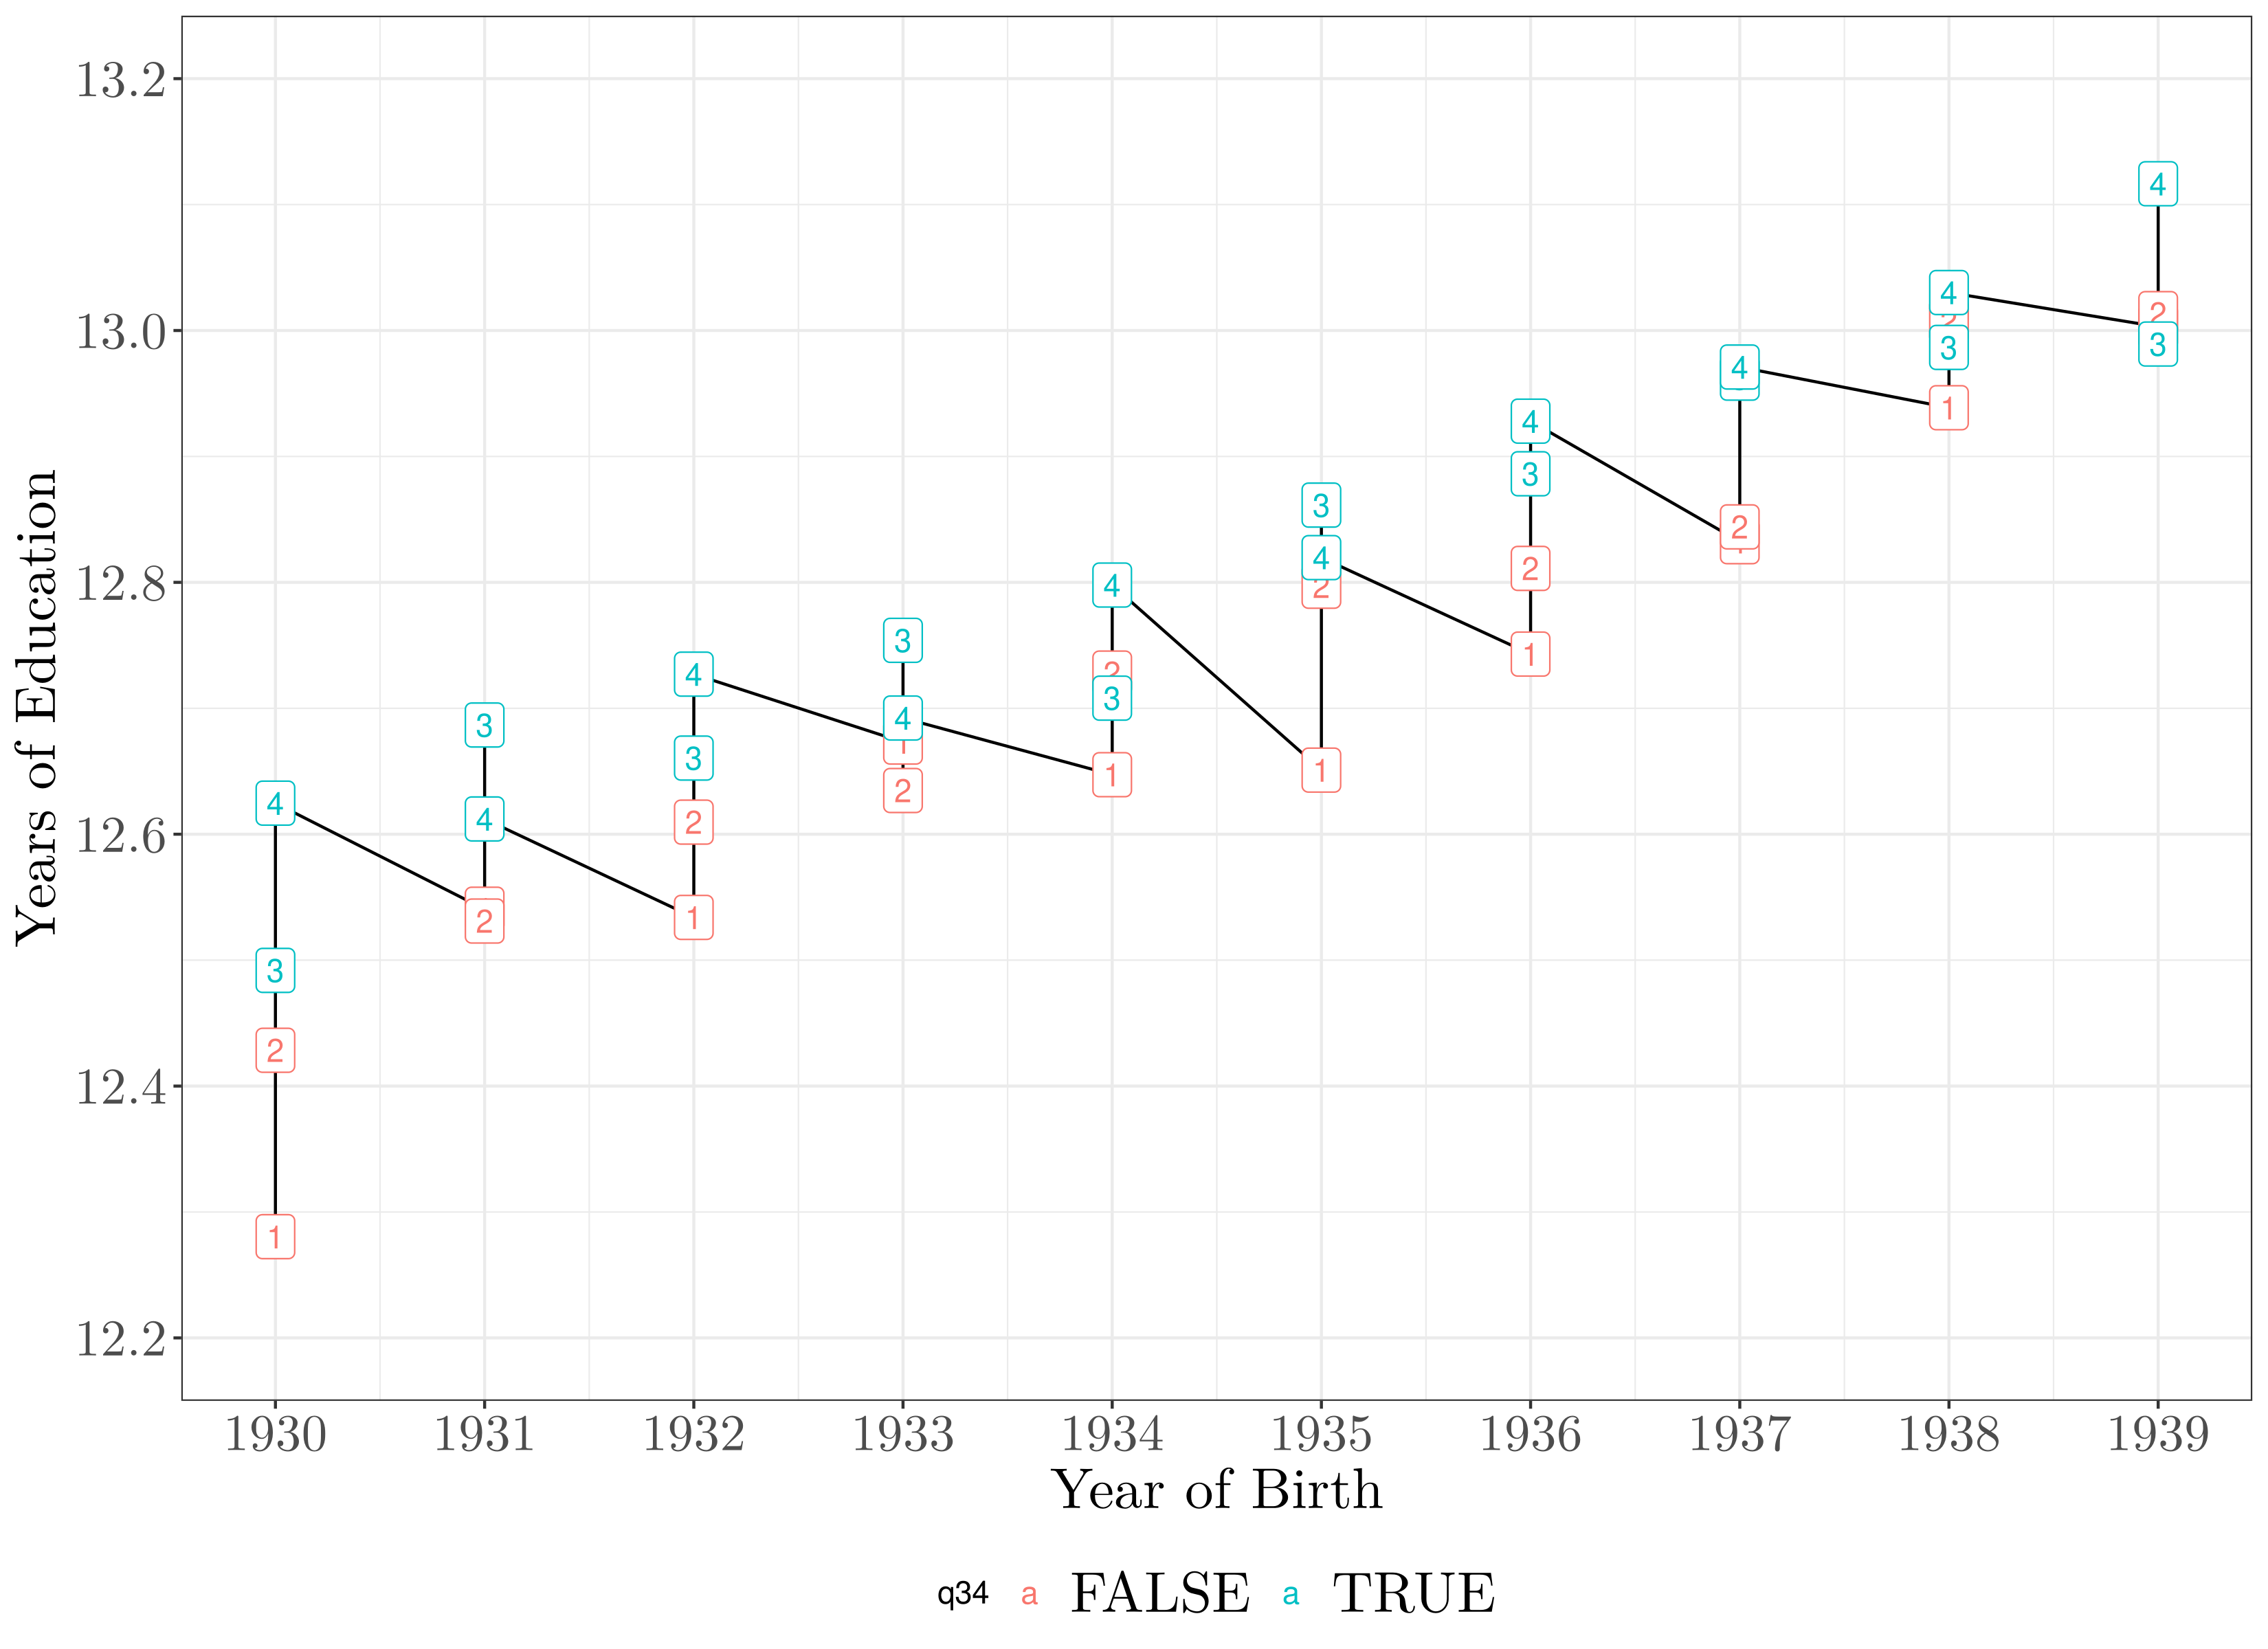
\includegraphics[scale=0.45]{"home/angelo/Documents/Uni/Courses/Advanced Statistics and programming/Assignments/assignment2/Graphics/task3_ivreg_proof.png"}
         \small
         \caption{Displaying association between Quarter of Birth and Years of Education}
\end{figure}

Finally, when considering Figure 2, one can seethat on average, Q4 and Q3 tend to have significantly more years of education than Q1 and Q2 - this might also explain the aforementioend results regarding Q2 difference to Q1 in model (4) in table 7. Overall, the instrument appears to meet the relevance criterion (ignoring cleanlisness etc here).\footnote{YOB seems to have a connection as well (see task 5)}






\begin{table}[!htbp] \centering 
\begin{adjustwidth}{0.cm}{-0cm}
\begin{threeparttable}
\small
\captionsetup{font=small, justification=raggedright,singlelinecheck=false}
\caption{\textsc{First Stage regression output - Relevancy}}
\centering 
  \label{}
\small 
\begin{tabular}{@{\extracolsep{25pt}}lcccc} 
\\[-5.8ex]\hline 
\hline \\[-1.8ex] 
 & \multicolumn{4}{c}{\textit{Dependent variable:}} \\ 
\cline{2-5} 
\\[-1.8ex] & \multicolumn{4}{c}{educ} \\ 
\\[-1.8ex] & (1 - numeric) & (2 - numeric) & (3 - categorical) & (4 - categorical)\\ 
\hline \\[-1.8ex] 
 Constant & 12.641$^{***}$ & 15.150$^{***}$ & 12.688$^{***}$ & 15.213$^{***}$ \\ 
  & (0.014) & (0.091) & (0.011) & (0.091) \\ 
  qob & 0.052$^{***}$ & 0.032$^{***}$ &  &  \\ 
  & (0.005) & (0.005) &  &  \\ 
  age &  & $-$0.060$^{***}$ &  & $-$0.060$^{***}$ \\ 
  &  & (0.002) &  & (0.002) \\ 
  married &  & 0.248$^{***}$ &  & 0.248$^{***}$ \\ 
  &  & (0.017) &  & (0.017) \\ 
  qob\_fac2 &  &  & 0.057$^{***}$ & $-$0.004 \\ 
  &  &  & (0.016) & (0.016) \\ 
  qob\_fac3 &  &  & 0.117$^{***}$ & 0.052$^{***}$ \\ 
  &  &  & (0.016) & (0.016) \\ 
  qob\_fac4 &  &  & 0.151$^{***}$ & 0.088$^{***}$ \\ 
  &  &  & (0.016) & (0.016) \\ 
 \hline \\[-1.8ex] 
Observations & 329,509 & 329,509 & 329,509 & 329,509 \\ 
R$^{2}$ & 0.0003 & 0.004 & 0.0003 & 0.004 \\ 
Adjusted R$^{2}$ & 0.0003 & 0.004 & 0.0003 & 0.004 \\ 
Residual Std. Error & 3.281 & 3.275 & 3.281  & 3.275  \\ 
F Statistic & 100.653$^{***}$  & 414.645$^{***}$ & 34.009$^{***}$ & 249.859$^{***}$  \\ 
\hline 
\hline \\[-3.5ex] 
\end{tabular} 
\begin{tablenotes}[para,flushleft]
      \small
      \item\textit{Note:} N = 329,509 - degrees of freedom are not reported for F tests; *** p$<$0.01, ** p$<$0.05, * p$<$0.1
    \end{tablenotes}
\end{threeparttable}
\end{adjustwidth}
%
\end{table}





\subsection{Task 4: Conduct IVreg of the effect of effect of education on log wages, using quarter of birth as the instrument; are robust SE needed?}
For the purpose of this analysis, it is assumed that the control variables are all exogenous. Table 8 reports the corresponding outputs; model (1) and (3) consider qob as a numeric variable and model (2) and (4) consider it as a categorical variable.\footnote{It may be noted that qob should be interpreted as a categorical variable in actuality.} Models (5) and (6) consider an additional instrument (discussed in part 5).
The control variables chosen are SMSA and whether married or not. Married was included because the proportion of married men tends to be higher for higher educated men, suggesting more education but also more income. Moreover, SMSA indicates whether a person lives in a rural or urban surrounding; people in urban areas may have better access to education and better work opportunities.
Considering the base models (1 - numeric) and (2 - categorical), we can observe that the choice between qob as a numeric or categorical variable instrument barely changes the coefficients and standard errors; reporting a significant positive coefficient for the years of education coefficient (model 1: $\hat{\beta}$ = 0.099, $p$ $<$ 0.01; model 2: $\hat{\beta}$ = 0.103, $p$ $<$ 0.01). For example, for model (2), this implies that one year more we can see that if education increases by one year wage increases by 10.3\%. 

Moving to model (4 - categorical), which contains SMSA and married as exogenous controls, the direction and magnitude, in addition to reported standard errors, for years of education do not change considerably when compared to model (2) (same for model 3 and 1), reporting a significant positive coefficient for education ($\hat{\beta}$ = 0.100, $p$ $<$ 0.01). Meaning, that an increase by one year in years of education is associated with a 10\% higher wage. Also the control variables are significant which are both categorical (SMSA: $\hat{\beta}$ = -0.148, $p$ $<$ 0.01; married: $\hat{\beta}$ = -0.255, $p$ $<$ 0.01); However, due to them being controls, we refrain from interpreting them here as we did with education. Thus, the inclusion of (assumed) exogenous controls does not impact change insights derived from the model.

Regarding robustness, the Breusch Pagan test was significant at conventional levels for all six models (not surprising at this sample size), suggesting no issues regarding heteroscedasticity. Moreover, when applying (White) standard errors, the non standardized standard errors maintain stability , suggesting that this research is not suffering from heteroscedasticity (see Appendix Table 16). Finally, an analysis of the (Residual Distribution) QQ Plot of model (4) (see Appendix Figure 3) also do not suggest extreme deviations in the residuals from a constant. Thus, statistical inference is not impacted by the inclusion of robust standard errors. 



% Table created by stargazer v.5.2.3 by Marek Hlavac, Social Policy Institute. E-mail: marek.hlavac at gmail.com
% Date and time: Thu, Sep 29, 2022 - 12:17:17
\begin{table}[!htbp] \centering 
\begin{adjustwidth}{0.cm}{-0cm}
\begin{threeparttable}
\small
\captionsetup{font=small, justification=raggedright,singlelinecheck=false}
\caption{\textsc{IV regression output}}
\centering 
  \label{}
\small 
\begin{tabular}{@{\extracolsep{-3pt}}lcccccc} 
\\[-5.8ex]\hline 
\hline \\[-1.8ex] 
 & \multicolumn{6}{c}{\textit{Dependent variable:}} \\ 
\cline{2-7} 
\\[-1.8ex] & \multicolumn{6}{c}{lnwage} \\ 
\\[-1.8ex] & (1 numeric) & (2 categorical) & (3 numeric) & (4 categorical) & (5 numeric) & (6 categorical)\\ 
\hline \\[-1.8ex] 
 Constant & 4.633$^{***}$ & 4.590$^{***}$ & 4.461$^{***}$ & 4.425$^{***}$ & 5.514$^{***}$ & 5.511$^{***}$ \\ 
  & (0.250) & (0.249) & (0.249) & (0.248) & (0.076) & (0.076) \\ 
  educ & 0.099$^{***}$ & 0.103$^{***}$ & 0.098$^{***}$ & 0.100$^{***}$ & 0.015$^{**}$ & 0.015$^{**}$ \\ 
  & (0.020) & (0.020) & (0.020) & (0.019) & (0.006) & (0.006) \\ 
  SMSA &  &  & $-$0.151$^{***}$ & $-$0.148$^{***}$ & $-$0.243$^{***}$ & $-$0.243$^{***}$ \\ 
  &  &  & (0.022) & (0.022) & (0.007) & (0.007) \\ 
  married &  &  & 0.256$^{***}$ & 0.255$^{***}$ & 0.280$^{***}$ & 0.280$^{***}$ \\ 
  &  &  & (0.006) & (0.006) & (0.004) & (0.004) \\ 
 \hline \\[-1.8ex] 
Observations & 329,509 & 329,509 & 329,509 & 329,509 & 329,509 & 329,509 \\ 
R$^{2}$ & 0.098 & 0.094 & 0.124 & 0.120 & 0.082 & 0.083 \\ 
Adjusted R$^{2}$ & 0.098 & 0.094 & 0.124 & 0.120 & 0.082 & 0.083 \\ 
Residual Std. Error & 0.645  & 0.646  & 0.635  & 0.637 & 0.650 & 0.650  \\ 
\hline 
\hline \\[-3.5ex] 
\end{tabular} 
\begin{tablenotes}[para,flushleft]
      \small
      \item\textit{Note:} N = 329,509 - degrees of freedom are not reported for F tests. SMSA comparison category is rural; married comparison category is not maried. *** p$<$0.01, ** p$<$0.05, * p$<$0.1.
    \end{tablenotes}
\end{threeparttable}
\end{adjustwidth}
%
\end{table}



\subsection{Task 5: Manual OLS and Selection}

% Table created by stargazer v.5.2.3 by Marek Hlavac, Social Policy Institute. E-mail: marek.hlavac at gmail.com
% Date and time: Thu, Sep 29, 2022 - 17:18:36
\begin{table}[!htbp] \centering 
\begin{adjustwidth}{0.cm}{-0cm}
\begin{threeparttable}
\small
\captionsetup{font=small, justification=raggedright,singlelinecheck=false}
\caption{\textsc{IV regression output Manual}}
\centering 
  \label{}
\small 
\begin{tabular}{@{\extracolsep{-4pt}}lcccccc} 
\\[-5.8ex]\hline 
\hline \\[-1.8ex] 
 & \multicolumn{6}{c}{\textit{Dependent variable:}} \\ 
\cline{2-7} 
\\[-1.8ex] & \multicolumn{6}{c}{lnwage} \\ 
\\[-1.8ex] & OLS (1) & OLS (2) & ManualIV(3) & ManualIV(4) & ManualIV(5) & ManualIV(6)\\ 
\hline \\[-1.8ex] 
 Constant & 4.995$^{***}$ & 4.847$^{***}$ & 4.633$^{***}$ & 4.461$^{***}$ & 4.590$^{***}$ & 4.425$^{***}$ \\ 
  & (0.004) & (0.005) & (0.263) & (0.260) & (0.262) & (0.259) \\ 
  educ & 0.071$^{***}$ & 0.067$^{***}$ &  &  &  &  \\ 
  & (0.0003) & (0.0003) &  &  &  &  \\ 
  SMSA &  & $-$0.185$^{***}$ &  & $-$0.151$^{***}$ &  & $-$0.148$^{***}$ \\ 
  &  & (0.003) &  & (0.023) &  & (0.023) \\ 
  married &  & 0.265$^{***}$ &  & 0.256$^{***}$ &  & 0.255$^{***}$ \\ 
  &  & (0.003) &  & (0.007) &  & (0.007) \\ 
  educ.hat &  &  & 0.099$^{***}$ & 0.098$^{***}$ & 0.103$^{***}$ & 0.100$^{***}$ \\ 
  &  &  & (0.021) & (0.020) & (0.020) & (0.020) \\ 
 \hline \\[-1.8ex] 
Observations & 329,509 & 329,509 & 329,509 & 329,509 & 329,509 & 329,509 \\ 
R$^{2}$ & 0.117 & 0.145 & 0.0001 & 0.041 & 0.0001 & 0.041 \\ 
Adjusted R$^{2}$ & 0.117 & 0.145 & 0.0001 & 0.041 & 0.0001 & 0.041 \\ 
Residual Std. Error & 0.638 & 0.628 & 0.679 & 0.665  & 0.679& 0.665  \\ 
F Statistic & 43,782.560$^{***}$ & 18,646.640$^{***}$  & 23.145$^{***}$  & 4,738.984$^{***}$ & 25.088$^{***}$ & 4,739.535$^{***}$ \\ 
\hline 
\hline \\[-3.5ex] 
\end{tabular} 
\begin{tablenotes}[para,flushleft]
      \small
      \item\textit{Note:} *** p$<$0.01, ** p$<$0.05, * p$<$0.1.
    \end{tablenotes}
\end{threeparttable}
\end{adjustwidth}
%
\end{table}

Note: this question was not precise wrt. whether to run a manual 2SLS or just normal OLS.

Model (1) and (2) in Table 9 report the OLS regressions of lnwage on the endogenous education with and without covariates. Models (3) and (4) report the manual 2SLS for quarter of birth as a numeric. Models (5) and (6) report quarter of birth as a factor. 

\indent Considering model (2), standard OLS with covariates, the overall effect of education on is significantly positive ($\hat{\beta}$ = 0.067, $p$ $<$ 0.01), which does not deviate drastically from its (assumed) exogenous counterpart in the other models in Table 8 (and 9). However, we can observe a considerably lower standard error for the years of education coefficient in model (2) when compared to Table 8 models 1 through 6.

\indent Moving on now to the manual 2SLS, as expected, the reported coefficients in models 3 through 6 in Table 9 correspond exactly with those reported in Table 8 (models 1 through 4). However, the manual 2SLS does not correct for the fact that years of education (hat) originates as a predicted outcome of the first stage. Thus, the standard errors differ slightly.

\indent Considering how which model to prefer, OLS vs model of methods or IVREG, the Hausman's ${\chi}^2$ can be used to assess which estimator is to be preferred. These are output from R directly, together with a test for weak instruments and, in case of over identification, the Sargan-Hansen ${\chi}^2$ over-identification test (there is no true test of exogenity). To keep it short, two models are considered for demonstrative purposes: 1) Table 8 model (3) where qob is a numeric variable (so no over-identification), and 2) Table 8 model (5) is considered where $yob$ (year of birth) was added as an instrument to demonstrate over identification. Please note that technically, the inclusion of qob as a factor implies over-identification of the first stage; this will be ignored in this question.

\indent Considering Table 10 and 11, the weak instruments test, which is just a partial F-test on the first stage of 2SLS, reports significant F statistics for both models (model 3: $F Statistic$ = 100.159, $p$ $<$ 0.01; model 5:$F Statistic$ = 557.21, $p$ $<$ 0.01), suggesting that the relevance criterion is fulfilled. Moving to the Wu-Hausman test however, the models differ. Model (3) (qob numeric model) reports and insignificant test statistic (${\chi}^2$ = 2.477, $p$ = 0.116), suggesting a preference for the OLS estimator. Contrarily, Model (5) reports a significant test statistic (${\chi}^2$ = 82.16), suggesting that the usage of model of methods (2SLS) is preferred over OLS in this case.\footnote{Please note that I included this example on purpose} Finally, considering the question of over-identification, this is not applicable to model (3), when considering qob as a numeric; it would, however, be relevant if we considered qob as a factor. Model (5), on the other hand, contains a second instrument, year of birth, as a demonstrative example. As can be seen in Table 10, the Sargan-Hansen ${\chi}^2$ test of over-identification reports a significant test statistic (${\chi}^2$ = 18.84, $p$ $<$ 0.01). Rejecting the null hypothesis implies that independence of the instruments of the residuals cannot be assumed. Thus, the instruments themselves are assumed to be endogenous themselves and over-identification poses a problem for model (5). It may be interesting to note that if we considered qob as a factor and only use it as a n instrument, this test statistic would be insignificant, suggesting that the qob as a factor is exogenous and, thus, over-identification is no problem. 



% latex table generated in R 4.1.3 by xtable 1.8-4 package
% Fri Sep 30 00:06:01 2022
\begin{table}[ht]
\captionsetup{font=small, justification=centering,singlelinecheck=false}
\caption{\textsc{IV Tests - QOB only}}
\centering
\begin{tabular}{rrrrr}
  \hline
 & df1 & df2 & statistic & p-value \\ 
  \hline
Weak instruments & 1.00 & 329505.00 & 100.16 & 0.00 \\ 
  Wu-Hausman & 1.00 & 329504.00 & 2.48 & 0.12 \\ 
  Sargan & 0.00 &  &  &  \\ 
   \hline
\end{tabular}
\end{table}

% latex table generated in R 4.1.3 by xtable 1.8-4 package
% Fri Sep 30 00:04:18 2022
\begin{table}[ht]
\captionsetup{font=small, justification=centering,singlelinecheck=false}
\caption{\textsc{IV Tests Overidentified}}
\centering
\begin{tabular}{rrrrr}
  \hline
 & df1 & df2 & statistic & p-value \\ 
  \hline
Weak instruments & 2.00 & 329504.00 & 557.21 & 0.00 \\ 
  Wu-Hausman & 1.00 & 329504.00 & 82.16 & 0.00 \\ 
  Sargan & 1.00 &  & 18.84 & 0.00 \\ 
   \hline
\end{tabular}
\end{table}

\subsection{Task 6: Cleanliness of the Instrument}
There are multiple ways which could invalidate the instrumental variable identification strategy invalid. 1) the instrument may not be relevant for the endogenous variable; it is notable that correlation does not necessarily guarantee relevance. Thus, it might actually be the case that qob is just not a relevant instrument and that the correlation is not strong enough - but that was dealt with in task 3. 2) The (supposed) variable years of education is actually not endogenous; remember that this is mostly based on theory and not on tests. 

However, the most interesting point to discuss considers 3) the cleanliness of the instrument. This would mean, that qob does not only have an effect on lnwage through the endogenous variable alone, but rather is a confounder itself, thus, having an impact on lnwage at the same time. One such case might be the developmental state of the child in question - meaning that eg. people from the first and second quarter, though having on average fewer years of education than people born in quarter third and fourth quarter, might still be "further" in terms of mental development at that time. This might lead to higher earnings for those older children and, thereby, relate the instrument to earnings. Thus, the assumption of cleanliness would be invalid.

Finally, 4) the instrument is endogenous itself, i.e. not mean independent - the instrument would be opening up further backdoor paths. A good example is that my father was born on the 11th of September but was only registered one month later; late registration would incur a fee (true story). Thus, in rural communities, non compliance with this specific requirement might be lacking. As such, qob would suffer from measurement error, particularly in the US during the 1930s. This would imply that qob is conditionally related to the error term and, thus, endogenous. Endogenous instruments themselves bias the resulting coefficient. 











\section{Bibliography}
\begin{thebibliography}{9}

\bibitem{ecitextbook}
@book{morgan2015counterfactuals,
  title={Counterfactuals and causal inference},
  author={Morgan, Stephen L and Winship, Christopher},
  year={2015},
  publisher={Cambridge University Press}
}

\indent Hlavac, M. (2018). $stargazer: Well-Formatted Regression and Summary Statistics Tables.$ Central European Labour Studies Institute (CELSI). https://CRAN.R-project.org/package=stargazer

\indent $Housing Prices Competition for Kaggle Learn Users, Dean De Cock$. (n.d.). Retrieved September 14, 2022, from https://www.kaggle.com/c/home-data-for-ml-course/data?select=train.csv

\indent Morgan, S. L., \& Winship, C. (2015). $Counterfactuals and causal inference.$ Cambridge University Press.


\indent  R Core Team (2013). R: A language and environment for statistical
  computing. R Foundation for Statistical Computing, Vienna, Austria.
  URL http://www.R-project.org/.
  
\indent Wickham H, Averick M, Bryan J, Chang W, McGowan LD, François R, Grolemund G, Hayes A, Henry L, Hester J, Kuhn M, Pedersen TL, Miller E, Bache SM, Müller K, Ooms J, Robinson D, Seidel DP, Spinu V, Takahashi K, Vaughan D, Wilke C, Woo K, Yutani H (2019). “Welcome to the tidyverse.” $Journal of Open Source Software$, 4(43), 1686. $doi:10.21105/joss.01686.$

Wickham H (2007). “Reshaping Data with the reshape Package.” $Journal of Statistical Software$, 21(12), 1–20. http://www.jstatsoft.org/v21/i12/.





\end{thebibliography}

\section{Appendix}


% Table created by stargazer v.5.2.3 by Marek Hlavac, Social Policy Institute. E-mail: marek.hlavac at gmail.com
% Date and time: Fri, Sep 23, 2022 - 20:47:48
\begin{table}[!htbp] 
\begin{adjustwidth}{-0cm}{-0cm}
\begin{threeparttable}
\small
\captionsetup{font=small, justification=raggedright,singlelinecheck=false}
  \caption{Descriptive Statistics of ECIC; With Children} 
  \label{} 
\begin{tabular}{@{\extracolsep{5pt}}lccccccc} 
\\[-1.8ex]\hline 
\hline \\[-1.8ex] 
Statistic & \multicolumn{1}{c}{Mean} & \multicolumn{1}{c}{St. Dev.} & \multicolumn{1}{c}{Min} & \multicolumn{1}{c}{Pctl(25)} & \multicolumn{1}{c}{Median} & \multicolumn{1}{c}{Pctl(75)} & \multicolumn{1}{c}{Max} \\ 
\hline \\[-1.8ex] 
Family Income & 12,750.390 & 15,739.050 & 0.000 & 4,652.465 & 8,425.197 & 15,218.720 & 410,507.600 \\ 
Earnings & 7,909.934 & 14,956.930 & 0.000 & 0.000 & 1,110.727 & 11,107.270 & 366,095.500 \\ 
Age & 32.717 & 8.630 & 20 & 25 & 32 & 39 & 54 \\ 
Education & 9.001 & 2.408 & 0 & 7 & 10 & 11 & 11 \\ 
Education Years & 4.840 & 5.872 & 0.000 & 0.071 & 3.761 & 7.070 & 102.958 \\ 
Unearned Income & 2.097 & 1.209 & 1 & 1 & 2 & 3 & 9 \\ 
Count Children & 0.466 & 0.499 & 0 & 0 & 0 & 1 & 1 \\ 
\hline \\[-1.8ex] 
\end{tabular} 
\begin{tablenotes}[para,flushleft]
      \small
      \item\textit{Notes:} N = 7819
    \end{tablenotes}
\end{threeparttable}
\end{adjustwidth}
\end{table} 




% Table created by stargazer v.5.2.3 by Marek Hlavac, Social Policy Institute. E-mail: marek.hlavac at gmail.com
% Date and time: Fri, Sep 23, 2022 - 20:47:48
\begin{table}[!htbp] 
\begin{adjustwidth}{-0cm}{-0cm}
\begin{threeparttable}
\small
\captionsetup{font=small, justification=raggedright,singlelinecheck=false}
  \caption{Descriptive Statistics of ECIC; Without Children} 
  \label{} 
\begin{tabular}{@{\extracolsep{5pt}}lccccccc} 
\\[-1.8ex]\hline 
\hline \\[-1.8ex] 
Statistic & \multicolumn{1}{c}{Mean} & \multicolumn{1}{c}{St. Dev.} & \multicolumn{1}{c}{Min} & \multicolumn{1}{c}{Pctl(25)} & \multicolumn{1}{c}{Median} & \multicolumn{1}{c}{Pctl(75)} & \multicolumn{1}{c}{Max} \\ 
\hline \\[-1.8ex] 
Family Income & 18,559.860 & 23,041.780 & 0.000 & 5,793.092 & 11,912.950 & 24,391.010 & 575,616.800 \\ 
Earnings & 13,760.260 & 21,301.400 & 0.000 & 0.000 & 7,664.014 & 19,447.610 & 537,880.600 \\ 
Age & 38.498 & 11.046 & 20 & 28 & 40 & 49 & 54 \\ 
Education & 8.549 & 2.889 & 0 & 7 & 10 & 11 & 11 \\ 
Education Years & 4.800 & 8.496 & 0.000 & 0.000 & 1.248 & 6.528 & 134.058 \\ 
Unearned Income & 0.000 & 0.000 & 0 & 0 & 0 & 0 & 0 \\ 
Count Children & 0.574 & 0.494 & 0 & 0 & 1 & 1 & 1 \\ 
\hline \\[-1.8ex] 
\end{tabular} 
\begin{tablenotes}[para,flushleft]
      \small
      \item\textit{Notes:} N = 5927
    \end{tablenotes}
\end{threeparttable}
\end{adjustwidth}
\end{table}


% Table created by stargazer v.5.2.3 by Marek Hlavac, Social Policy Institute. E-mail: marek.hlavac at gmail.com
% Date and time: Wed, Sep 14, 2022 - 15:53:27
\begin{table}[!htbp] \centering 
\begin{adjustwidth}{0.cm}{-0cm}
\begin{threeparttable}
\small
\captionsetup{font=small, justification=raggedright,singlelinecheck=false}
\caption{\textsc{Non-Robust Regression Results Part 3}}
\centering 
  \label{}
\small 
\begin{tabular}{@{\extracolsep{-2pt}}lcccccc} 
\\[-5.8ex]\hline 
\hline \\[-1.8ex] 
 & \multicolumn{6}{c}{\textit{Dependent variable:}} \\ 
\cline{2-7} 
\\[-1.8ex] & \multicolumn{2}{c}{earn} & \multicolumn{2}{c}{finc} & \multicolumn{2}{c}{work} \\ 
\\[-1.8ex] & (1) & (2) & (3) & (4) & (5) & (6)\\ 
\hline \\[-1.8ex] 
 Constant & 14,899.900$^{***}$ & 12,958.640$^{***}$ & 20,099.430$^{***}$ & 16,218.430$^{***}$ & 0.582$^{***}$ & 0.532$^{***}$ \\ 
  & (828.375) & (1,550.012) & (886.522) & (1,655.347) & (0.023) & (0.043) \\ 
  has\_children1 & $-$8,596.327$^{***}$ & $-$8,394.973$^{***}$ & $-$8,929.330$^{***}$ & $-$8,269.567$^{***}$ & $-$0.159$^{***}$ & $-$0.150$^{***}$ \\ 
  & (1,093.444) & (1,096.506) & (1,170.197) & (1,171.022) & (0.030) & (0.030) \\ 
  dperiod & $-$695.997 & $-$536.491 & $-$940.239$^{*}$ & $-$515.553 & $-$0.005 & $-$0.024$^{*}$ \\ 
  & (485.413) & (500.046) & (519.486) & (534.028) & (0.013) & (0.014) \\ 
  age &  & 22.555 &  & 78.717$^{***}$ &  & 0.002$^{***}$ \\ 
  &  & (15.922) &  & (17.004) &  & (0.0004) \\ 
  urate &  & 133.948 &  & 372.861$^{***}$ &  & $-$0.018$^{***}$ \\ 
  &  & (114.614) &  & (122.403) &  & (0.003) \\ 
  ed &  & 66.337 &  & $-$125.305$^{**}$ &  & 0.017$^{***}$ \\ 
  &  & (59.579) &  & (63.628) &  & (0.002) \\ 
  nonwhite1 &  & $-$1,255.622$^{***}$ &  & $-$2,438.387$^{***}$ &  & $-$0.043$^{***}$ \\ 
  &  & (326.237) &  & (348.408) &  & (0.009) \\ 
  has\_children1:dperiod & 1,682.810$^{***}$ & 1,722.360$^{***}$ & 1,911.035$^{***}$ & 2,006.060$^{***}$ & 0.031$^{*}$ & 0.033$^{*}$ \\ 
  & (642.099) & (641.893) & (687.171) & (685.515) & (0.018) & (0.018) \\ 
 \hline \\[-1.8ex] 
R$^{2}$ & 0.026 & 0.027 & 0.022 & 0.028 & 0.012 & 0.027 \\ 
Adjusted R$^{2}$ & 0.026 & 0.027 & 0.022 & 0.027 & 0.012 & 0.026 \\ 
Residual Std. Error & 17,965.670 & 17,956.450  & 19,226.750  & 19,176.730 & 0.497  & 0.493  \\ 
F Statistic & 121.691$^{***}$ & 54.794$^{***}$ & 105.245$^{***}$ & 56.166$^{***}$  & 54.906$^{***}$  & 54.374$^{***}$  \\ 
\hline 
\hline \\[-3.5ex] 
\end{tabular} 
\begin{tablenotes}[para,flushleft]
      \small
      \item\textit{Note:} N = 13746. Non Robust Standard Errors applied. "White" is reference category for "non-White" categorical variable.
    \end{tablenotes}
\end{threeparttable}
\end{adjustwidth}
%
\end{table}

\begin{landscape}
% Table created by stargazer v.5.2.3 by Marek Hlavac, Social Policy Institute. E-mail: marek.hlavac at gmail.com
% Date and time: Wed, Sep 28, 2022 - 18:35:54
\begin{table}[!htbp] \centering 
\begin{adjustwidth}{1.25cm}{-0cm}
\begin{threeparttable}
\small
\captionsetup{font=small, justification=raggedright,singlelinecheck=false}
\caption{\textsc{Non-Robust Regression Results Part 3}}
\centering 
  \label{}
\small 
\begin{tabular}{@{\extracolsep{-2pt}}lccccccccc} 
\\[-5.8ex]\hline 
\hline \\[-1.8ex] 
 & \multicolumn{9}{c}{\textit{Dependent variable:}} \\ 
\cline{2-10} 
\\[-1.8ex] & \multicolumn{3}{c}{earn} & \multicolumn{3}{c}{finc} & \multicolumn{3}{c}{work} \\ 
\\[-1.8ex] & Basic(1) & White(2) & Cluster(3) & Basic(4) & White(5) & Cluster(6) & Basic(7) & White(8) & Cluster(9)\\ 
\hline \\[-1.8ex] 
 has\_children1 & $-$8,394.973$^{***}$ & $-$8,394.973$^{***}$ & $-$8,394.973$^{***}$ & $-$8,269.567$^{***}$ & $-$8,269.567$^{***}$ & $-$8,269.567$^{***}$ & $-$0.150$^{***}$ & $-$0.150$^{***}$ & $-$0.150$^{***}$ \\ 
  & (1,096.506) & (1,056.274) & (1,057.069) & (1,171.022) & (1,146.704) & (1,147.577) & (0.030) & (0.030) & (0.030) \\ 
  & & & & & & & & & \\ 
 dperiod & $-$536.491 & $-$536.491 & $-$536.491 & $-$515.553 & $-$515.553 & $-$515.553 & $-$0.024$^{*}$ & $-$0.024$^{*}$ & $-$0.024$^{*}$ \\ 
  & (500.046) & (564.674) & (565.075) & (534.028) & (618.997) & (619.444) & (0.014) & (0.014) & (0.014) \\ 
  & & & & & & & & & \\ 
 age & 22.555 & 22.555 & 22.555 & 78.717$^{***}$ & 78.717$^{***}$ & 78.717$^{***}$ & 0.002$^{***}$ & 0.002$^{***}$ & 0.002$^{***}$ \\ 
  & (15.922) & (19.063) & (19.077) & (17.004) & (20.183) & (20.198) & (0.0004) & (0.0004) & (0.0004) \\ 
  & & & & & & & & & \\ 
 urate & 133.948 & 133.948 & 133.948 & 372.861$^{***}$ & 372.861$^{***}$ & 372.861$^{***}$ & $-$0.018$^{***}$ & $-$0.018$^{***}$ & $-$0.018$^{***}$ \\ 
  & (114.614) & (114.009) & (114.096) & (122.403) & (123.441) & (123.537) & (0.003) & (0.003) & (0.003) \\ 
  & & & & & & & & & \\ 
 ed & 66.337 & 66.337 & 66.337 & $-$125.305$^{**}$ & $-$125.305$^{*}$ & $-$125.305$^{*}$ & 0.017$^{***}$ & 0.017$^{***}$ & 0.017$^{***}$ \\ 
  & (59.579) & (59.876) & (59.937) & (63.628) & (67.467) & (67.538) & (0.002) & (0.002) & (0.002) \\ 
  & & & & & & & & & \\ 
 nonwhite1 & $-$1,255.622$^{***}$ & $-$1,255.622$^{***}$ & $-$1,255.622$^{***}$ & $-$2,438.387$^{***}$ & $-$2,438.387$^{***}$ & $-$2,438.387$^{***}$ & $-$0.043$^{***}$ & $-$0.043$^{***}$ & $-$0.043$^{***}$ \\ 
  & (326.237) & (341.701) & (341.929) & (348.408) & (368.776) & (369.027) & (0.009) & (0.009) & (0.009) \\ 
  & & & & & & & & & \\ 
 has\_children1:dperiod & 1,722.360$^{***}$ & 1,722.360$^{***}$ & 1,722.360$^{***}$ & 2,006.060$^{***}$ & 2,006.060$^{***}$ & 2,006.060$^{***}$ & 0.033$^{*}$ & 0.033$^{*}$ & 0.033$^{*}$ \\ 
  & (641.893) & (647.317) & (647.764) & (685.515) & (698.628) & (699.118) & (0.018) & (0.018) & (0.018) \\ 
  & & & & & & & & & \\ 
 Constant & 12,958.640$^{***}$ & 12,958.640$^{***}$ & 12,958.640$^{***}$ & 16,218.430$^{***}$ & 16,218.430$^{***}$ & 16,218.430$^{***}$ & 0.532$^{***}$ & 0.532$^{***}$ & 0.532$^{***}$ \\ 
  & (1,550.012) & (1,622.488) & (1,623.778) & (1,655.347) & (1,771.017) & (1,772.450) & (0.043) & (0.042) & (0.042) \\ 
  & & & & & & & & & \\ 
\hline \\[-1.8ex] 
Observations & 13,746 & 13,746 & 13,746 & 13,746 & 13,746 & 13,746 & 13,746 & 13,746 & 13,746 \\ 
R$^{2}$ & 0.027 & 0.027 & 0.027 & 0.028 & 0.028 & 0.028 & 0.027 & 0.027 & 0.027 \\ 
Adjusted R$^{2}$ & 0.027 & 0.027 & 0.027 & 0.027 & 0.027 & 0.027 & 0.026 & 0.026 & 0.026 \\ 
Residual Std. Error  & 17,956.450 & 17,956.450 & 17,956.450 & 19,176.730 & 19,176.730 & 19,176.730 & 0.493 & 0.493 & 0.493 \\ 
F Statistic  & 54.794$^{***}$ & 54.794$^{***}$ & 54.794$^{***}$ & 56.166$^{***}$ & 56.166$^{***}$ & 56.166$^{***}$ & 54.374$^{***}$ & 54.374$^{***}$ & 54.374$^{***}$ \\ 
\hline 
\hline \\[-3.5ex] 
\end{tabular} 
\begin{tablenotes}[para,flushleft]
      \small
      \item\textit{Note:} N = 13746. Robust Standard Errors applied. "White" is reference category for "non-White" categorical variable. *** p$<$0.01, ** p$<$0.05, * p$<$0.1.
    \end{tablenotes}
\end{threeparttable}
\end{adjustwidth}
%
\end{table}

\end{landscape}



% Table created by stargazer v.5.2.3 by Marek Hlavac, Social Policy Institute. E-mail: marek.hlavac at gmail.com
% Date and time: Thu, Sep 29, 2022 - 23:52:12
\begin{table}[!htbp] \centering 
\begin{adjustwidth}{1.25cm}{-0cm}
\begin{threeparttable}
\small
\captionsetup{font=small, justification=raggedright,singlelinecheck=false}
\caption{\textsc{White-Robust Regression Results QOB numeric only}}
\centering 
  \label{}
\small 
\begin{tabular}{@{\extracolsep{-2pt}}lcccccc} 
\\[-5.8ex]\hline 
\hline \\[-1.8ex] 
 & \multicolumn{6}{c}{\textit{Dependent variable:}} \\ 
\cline{2-7} 
\\[-1.8ex] & \multicolumn{6}{c}{lnwage} \\ 
\\[-1.8ex] & Basic(1) & White(2) & Basic(3) & White(4) & Basic(5) & White(6)\\ 
\hline \\[-1.8ex] 
 educ & 0.099$^{***}$ & 0.099$^{***}$ & 0.098$^{***}$ & 0.098$^{***}$ & 0.015$^{**}$ & 0.015$^{**}$ \\ 
  & (0.020) & (0.020) & (0.020) & (0.020) & (0.006) & (0.006) \\ 
  & & & & & & \\ 
 SMSA &  &  & $-$0.151$^{***}$ & $-$0.151$^{***}$ & $-$0.243$^{***}$ & $-$0.243$^{***}$ \\ 
  &  &  & (0.022) & (0.022) & (0.007) & (0.007) \\ 
  & & & & & & \\ 
 married &  &  & 0.256$^{***}$ & 0.256$^{***}$ & 0.280$^{***}$ & 0.280$^{***}$ \\ 
  &  &  & (0.006) & (0.007) & (0.004) & (0.004) \\ 
  & & & & & & \\ 
 Constant & 4.633$^{***}$ & 4.633$^{***}$ & 4.461$^{***}$ & 4.461$^{***}$ & 5.514$^{***}$ & 5.514$^{***}$ \\ 
  & (0.250) & (0.249) & (0.249) & (0.248) & (0.076) & (0.076) \\ 
  & & & & & & \\ 
\hline \\[-1.8ex] 
Observations & 329,509 & 329,509 & 329,509 & 329,509 & 329,509 & 329,509 \\ 
R$^{2}$ & 0.098 & 0.098 & 0.124 & 0.124 & 0.082 & 0.082 \\ 
Adjusted R$^{2}$ & 0.098 & 0.098 & 0.124 & 0.124 & 0.082 & 0.082 \\ 
Residual Std. Error & 0.645  & 0.645 & 0.635 & 0.635  & 0.650  & 0.650  \\ 
\hline 
\hline \\[-3.5ex] 
\end{tabular} 
\begin{tablenotes}[para,flushleft]
      \small
      \item\textit{Note:} *** p$<$0.01, ** p$<$0.05, * p$<$0.1.
    \end{tablenotes}
\end{threeparttable}
\end{adjustwidth}
%
\end{table}


\begin{figure}[htp]
		\centering
         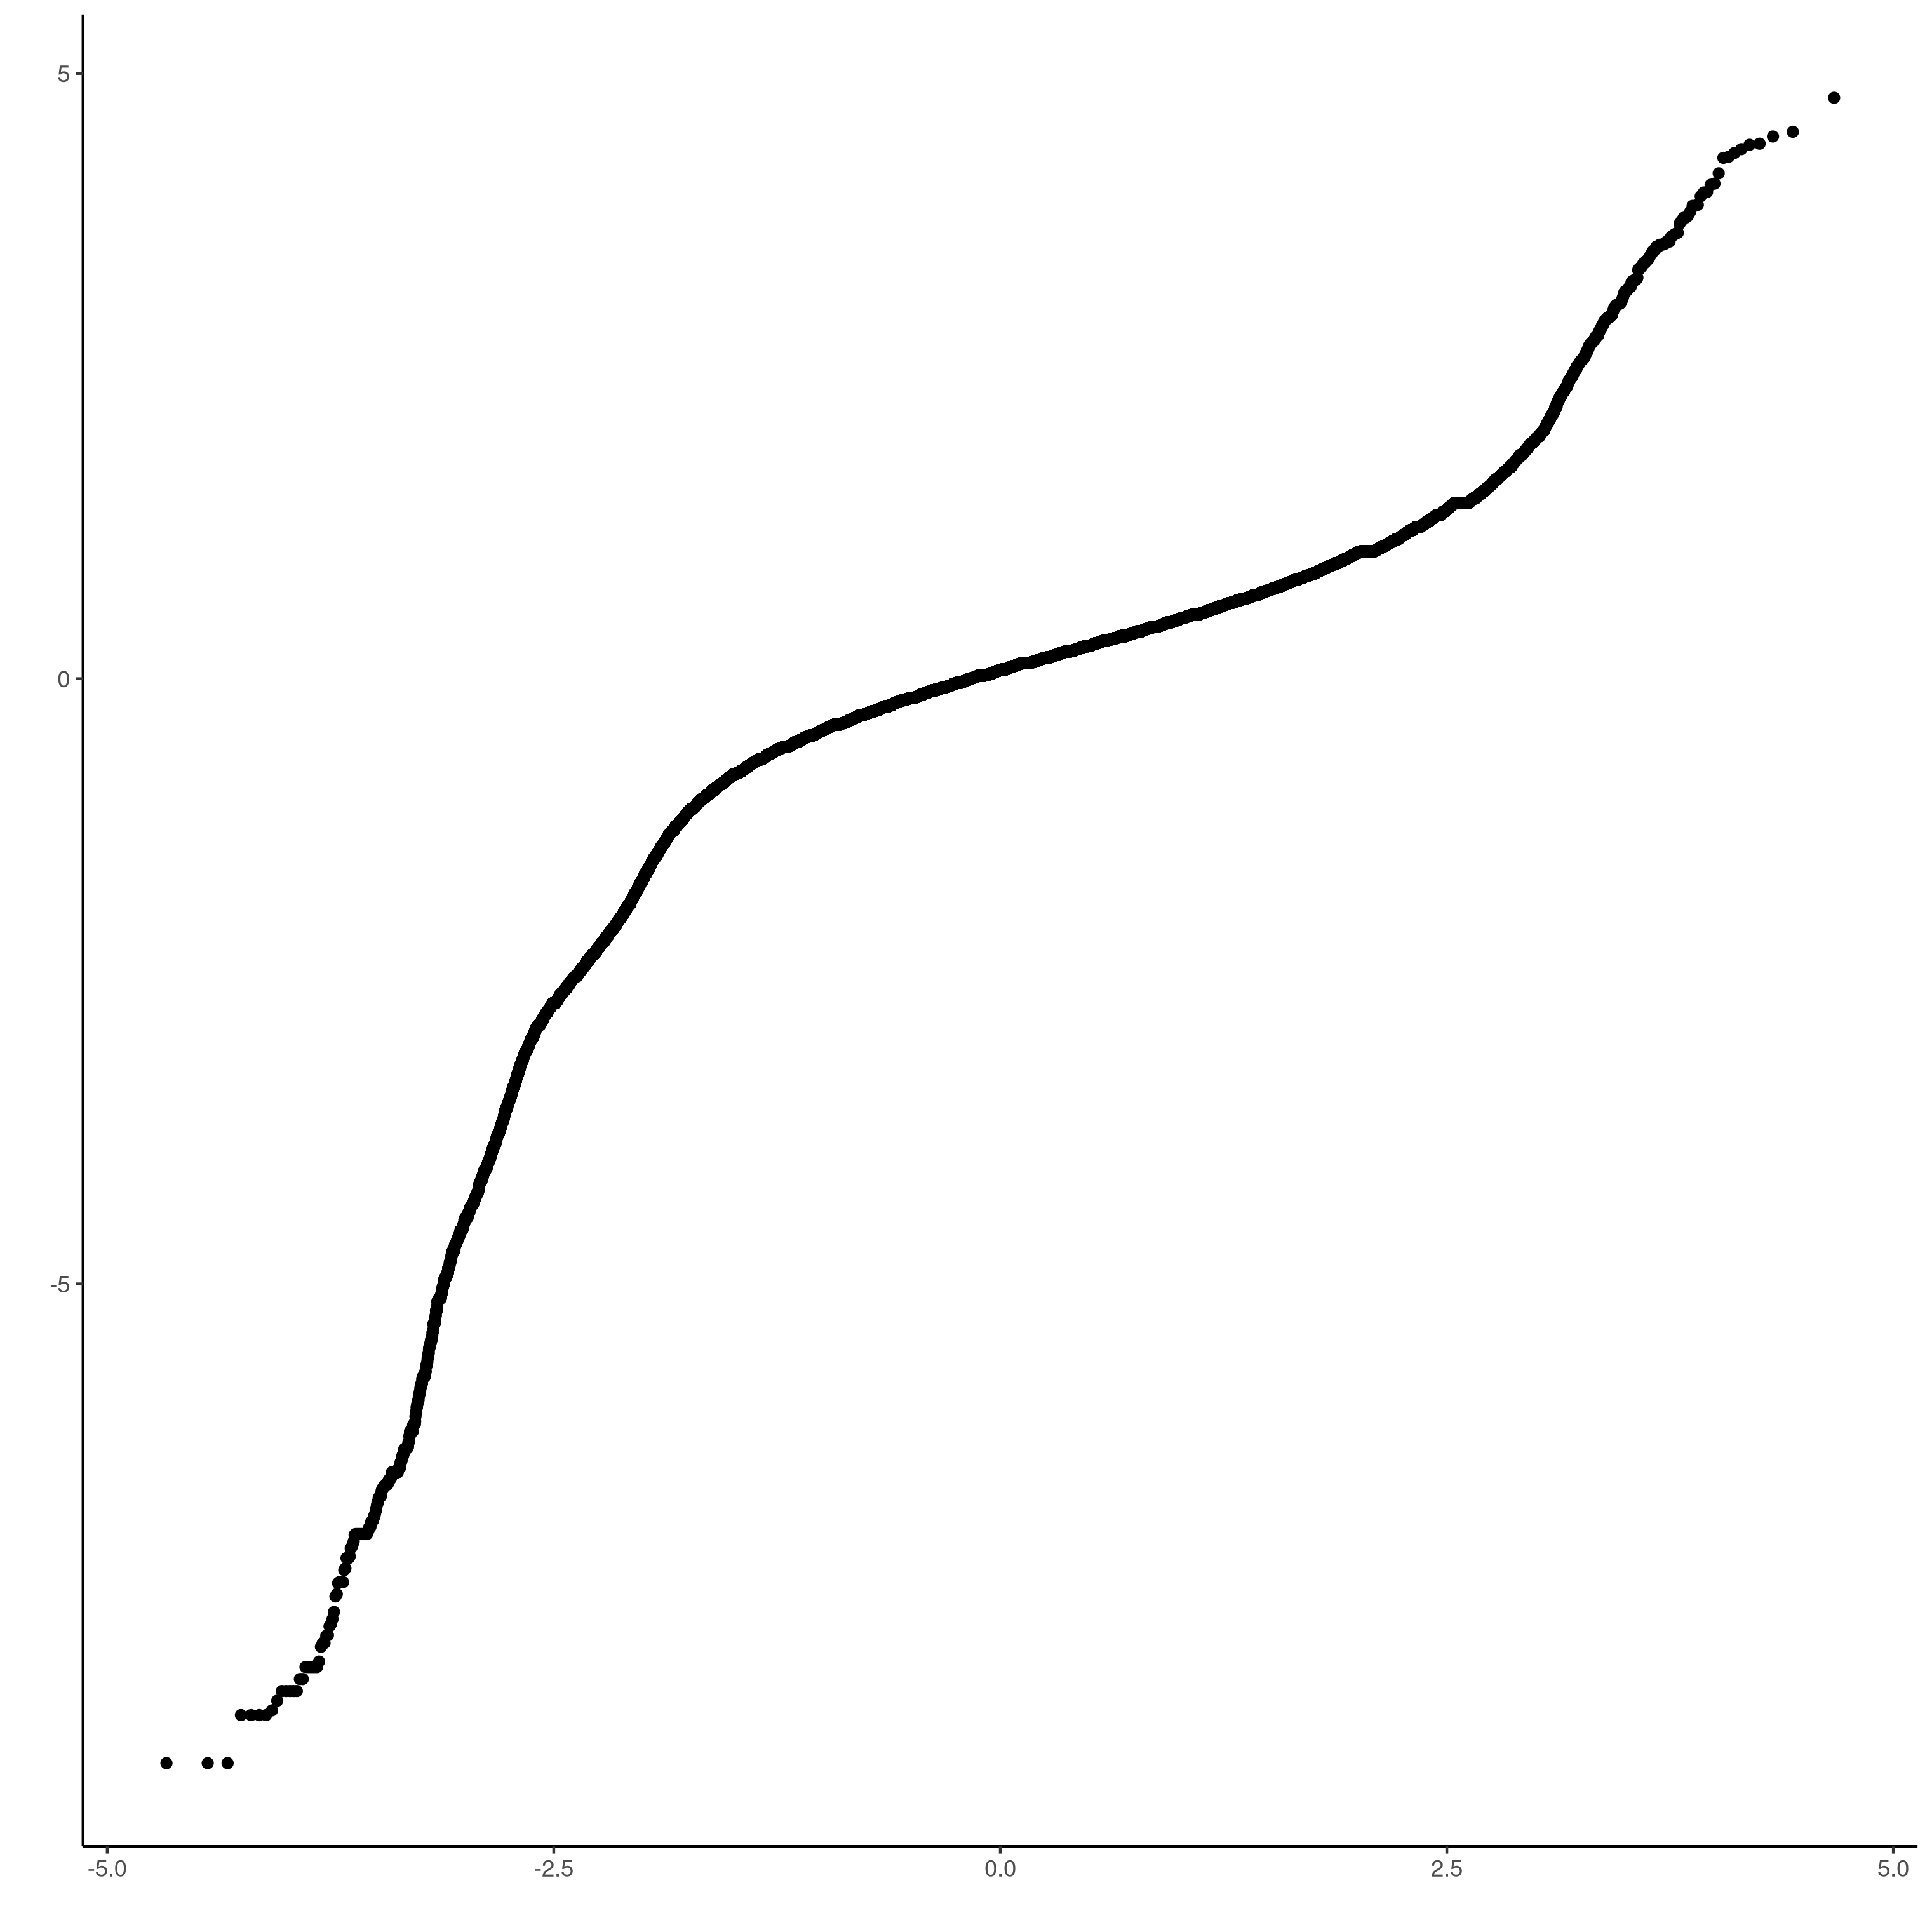
\includegraphics[scale=0.35]{"/home/angelo/Documents/Uni/Courses/Advanced Statistics and programming/Assignments/assignment2/Graphics/qqplots.png"}
         \small
         \caption{Residual Distribution Plot}
\end{figure}


\section{Code}

\begin{lstlisting}[language=R]

# clear environment
rm(list = ls())

# import the necessary libraries
library("tidyverse")
library("stargazer")
library("tidyverse")
library("reshape2")
library("Hmisc")
library("ggplot2")
library("dplyr")
library("moments")
library("lm.beta")
library("fastDummies")
library("stringr")
library("extrafont")
library("gridExtra")
library("AER")
library("DAAG")
loadfonts()





setwd("/home/angelo/Documents/Uni/Courses/Advanced Statistics and programming/Assignments/assignment2")

df <- read.csv("Data/DiD_dataset-1.csv", header = TRUE, sep = ",")

# indicate child or not
df <- df %>%
    mutate(has_children = case_when(
        children > 0 ~ TRUE,
        children == 0 ~ FALSE
    ))

# first set up indicator that whether treatment vs non treatment period
df <- df %>% mutate(dperiod = case_when(year < 1993 ~ 1, year >= 1993 ~ 2))

df$nonwhite <- as.factor(df$nonwhite)
df$state <- as.factor(df$state)
df$year <- as.factor(df$year)



#---------------------------------------------------------------------------------------
#---------------------------------------------------------------------------------------
# Task 2; plot 3 dependent variables;

# a) annual earnings (earn)
ggplot(df, aes(year, earn, group = has_children, color = has_children)) +
    stat_summary(geom = "line", fun = mean) +
    labs(x = "Year", y = "Earnings", color = "Has Children") +
    theme_minimal() +
    geom_vline(xintercept = "1993") +
    theme_set(theme_bw() + theme(legend.position = "bottom")) +
    theme(
        axis.text.x = element_text(size = 20, family = "LM Roman 10"),
        axis.text.y = element_text(size = 20, family = "LM Roman 10"),
        axis.title = element_text(size = 20, family = "LM Roman 10"),
        legend.text = element_text(size = 20, family = "LM Roman 10")
    )

ggsave("Graphics/task2_earn_did.png", width = 11, height = 8)

# b) annual family income (finc)
ggplot(df, aes(year, finc, group = has_children, color = has_children)) +
    stat_summary(geom = "line", fun = mean) +
    labs(x = "Year", y = "Family Income", color = "Has Children") +
    theme_minimal() +
    geom_vline(xintercept = "1993") +
    theme_set(theme_bw() + theme(legend.position = "bottom")) +
    theme(
        axis.text.x = element_text(size = 20, family = "LM Roman 10"),
        axis.text.y = element_text(size = 20, family = "LM Roman 10"),
        axis.title = element_text(size = 20, family = "LM Roman 10"),
        legend.text = element_text(size = 20, family = "LM Roman 10")
    )

ggsave("Graphics/task2_finc_did.png", width = 11, height = 8)

# c) working/non-working (work)
ggplot(df, aes(year, work, group = has_children, color = has_children)) +
    stat_summary(geom = "line", fun = mean) +
    labs(x = "Year", y = "Work Proportion", color = "Has Children") +
    theme_minimal() +
    geom_vline(xintercept = "1993") +
    theme_set(theme_bw() + theme(legend.position = "bottom")) +
    theme(
        axis.text.x = element_text(size = 20, family = "LM Roman 10"),
        axis.text.y = element_text(size = 20, family = "LM Roman 10"),
        axis.title = element_text(size = 20, family = "LM Roman 10"),
        legend.text = element_text(size = 20, family = "LM Roman 10")
    )

ggsave("Graphics/task2_work_did.png", width = 11, height = 8)


df <- df %>%
    mutate(has_children = case_when(
        children > 0 ~ 1,
        children == 0 ~ 0
    ))

#---------------------------------------------------------------------------------------
#---------------------------------------------------------------------------------------
# Task 3
df_temp <- df %>%
    select((c("finc", "earn", "age", "urate", "ed", "unearn", "children", "work")))

df_temp_w_children <- subset(
    df, has_children == TRUE
)

df_temp_w_children <- df_temp_w_children %>%
    select((c("finc", "earn", "age", "urate", "ed", "unearn", "children", "work")))

df_temp_wo_children <- subset(
    df, has_children == FALSE
)
View(df)
df_temp_wo_children <- df_temp_wo_children %>%
    select((c("finc", "earn", "age", "ed", "urate", "unearn", "children", "work")))

str(df_temp_w_children)


stargazer(
    df,
    type = "latex",
    # omit.summary.stat = c("N"),
    summary.stat = c("mean", "sd", "min", "p25", "median", "p75", "max"),
    title = "Descriptive Statistics of ECIC"

)
skewness(df$earn)
df %>% count(has_children)
table(df$nonwhite)
cor(df$earn, df$finc, )
stargazer(
    df_temp_w_children,
    type = "latex",
    omit.summary.stat = c("N"),
    summary.stat = c("mean", "sd", "min", "p25", "median", "p75", "max"),
    title = "Descriptive Statistics of ECIC; With Children",
    covariate.labels = c(
        "Family Income", "Earnings", "Age", "Education",
        "Education Years", "Unearned Income", "Count Children", "Work"
    )
)

stargazer(
    df_temp_wo_children,
    type = "latex",
    omit.summary.stat = c("N"),
    summary.stat = c("mean", "sd", "min", "p25", "median", "p75", "max"),
    title = "Descriptive Statistics of ECIC; Without Children",
    covariate.labels = c(
        "Family Income", "Earnings", "Age", "Education",
        "Education Years", "Unearned Income", "Count Children", "Work"
    )
)


#---------------------------------------------------------------------------------------
#---------------------------------------------------------------------------------------
# Task 4 - create the matrixes

# Find averages per year/dperiod in per earn, finc, work
df_g_summary <- df %>%
    group_by(dperiod, has_children) %>%
    summarise_at(vars(earn, finc, work), funs(mean(., na.rm = TRUE)), round = 2)

df_g_summary_earn <- df %>%
    group_by(dperiod, has_children) %>%
    summarise_at(vars(earn), funs(mean(., na.rm = TRUE)), round = 2)

df_g_summary_finc <- df %>%
    group_by(dperiod, has_children) %>%
    summarise_at(vars(finc), funs(mean(., na.rm = TRUE)), round = 2)

df_g_summary_work <- df %>%
    group_by(dperiod, has_children) %>%
    summarise_at(vars(work), funs(mean(., na.rm = TRUE)), round = 2)

df_g_summary

df_g_summary %>% separate_header(sep = "has_children")

# long to wide transformation
tmp_earn <- dcast(df_g_summary_earn, dperiod ~ has_children, value.var = c("earn"))
tmp_finc <- dcast(df_g_summary_finc, dperiod ~ has_children, value.var = c("finc"))
tmp_work <- dcast(df_g_summary_work, dperiod ~ has_children, value.var = c("work"))


tmp <- merge(tmp_earn, tmp_finc, by.x = "dperiod", by.y = "dperiod")
tmp <- merge(tmp, tmp_work, by.x = "dperiod", by.y = "dperiod")
tmp

tmp <- rbind(tmp, tmp[2, ] - tmp[1, ])
rownames(tmp) <- c("Before", "After", "Difference")
tmp[3, 1] <- NA
tmp


# round the output
tmp[, -1] <- round(tmp[, -1], 2)
tmp

# Make a table with the results
stargazer(tmp, summary = FALSE, align = TRUE, type = "text")

stargazer(tmp, summary = FALSE, align = TRUE, type = "latex")

#' df_g_summary


#---------------------------------------------------------------------------------------
#---------------------------------------------------------------------------------------
# Task 5 -

df <- df %>%
    mutate(has_children = case_when(
        children > 0 ~ 1,
        children == 0 ~ 0
    ))
df$has_children <- as.factor(df$has_children)


##################
# Earn models
cov_earn <- earn ~ age + urate + ed + nonwhite

did_earn_sim <- earn ~ has_children + dperiod + has_children:dperiod
did_earn_expand <- earn ~ has_children + dperiod + has_children:dperiod + age + urate + ed + nonwhite

rslt_earn_cov <- lm(cov_earn, data = df)
rsltdid_earn_sim <- lm(did_earn_sim, data = df)
rsltdid_earn_expand <- lm(did_earn_expand, data = df)


##################
# finc models
cov_finc <- finc ~ age + urate + ed + nonwhite

did_finc_sim <- finc ~ has_children + dperiod + has_children:dperiod
did_finc_expand <- finc ~ has_children + dperiod + has_children:dperiod + age + urate + ed + nonwhite

rslt_finc_cov <- lm(cov_finc, data = df)
rsltdid_finc_sim <- lm(did_finc_sim, data = df)
rsltdid_finc_expand <- lm(did_finc_expand, data = df)


##################
# work models
cov_work <- work ~ age + urate + ed + nonwhite

did_work_sim <- work ~ has_children + dperiod + has_children:dperiod
did_work_expand <- work ~ has_children + dperiod + has_children:dperiod + age + urate + ed + nonwhite

rslt_work_cov <- lm(cov_work, data = df)
rsltdid_work_sim <- lm(did_work_sim, data = df)
rsltdid_work_expand <- lm(did_work_expand, data = df)


stargazer(
    rsltdid_earn_sim,
    rsltdid_earn_expand,
    rsltdid_finc_sim,
    rsltdid_finc_expand,
    # rsltdid_work_sim,
    # rsltdid_work_expand,
    intercept.bottom = FALSE,
    align = TRUE,
    no.space = TRUE,
    # omit.labels = "Restaurant IDs?",
    type = "text"
)




stargazer(
    rslt_earn_cov,
    rsltdid_earn_sim,
    rsltdid_earn_expand,
    rslt_finc_cov,
    rsltdid_finc_sim,
    rsltdid_finc_expand,
    rslt_work_cov,
    rsltdid_work_sim,
    rsltdid_work_expand,
    intercept.bottom = FALSE,
    # align = TRUE,
    # no.space = TRUE,
    # omit.labels = "Restaurant IDs?",
    type = "latex"
)



#----------------------------------------

lmtest::bptest(rslt_earn_cov)
lmtest::bptest(rsltdid_earn_sim)
lmtest::bptest(rsltdid_earn_expand)

lmtest::bptest(rslt_finc_cov)
lmtest::bptest(rsltdid_finc_sim)
lmtest::bptest(rsltdid_finc_expand)

lmtest::bptest(rslt_work_cov)
lmtest::bptest(rsltdid_work_sim)
lmtest::bptest(rsltdid_work_expand)








# implement robust standard errors
seBasic <- sqrt(diag(vcov(rsltdid_earn_expand)))
seWhite <- sqrt(diag(vcovHC(rsltdid_earn_expand, type = "HC0")))
seClust <- sqrt(diag(vcovHC(rsltdid_earn_expand, cluster = "state")))

seBasic1 <- sqrt(diag(vcov(rsltdid_finc_expand)))
seWhite1 <- sqrt(diag(vcovHC(rsltdid_finc_expand, type = "HC0")))
seClust1 <- sqrt(diag(vcovHC(rsltdid_finc_expand, cluster = "state")))

seBasic2 <- sqrt(diag(vcov(rsltdid_work_expand)))
seWhite2 <- sqrt(diag(vcovHC(rsltdid_work_expand, type = "HC0")))
seClust2 <- sqrt(diag(vcovHC(rsltdid_work_expand, cluster = "state")))



stargazer(rsltdid_earn_expand, rsltdid_earn_expand, rsltdid_earn_expand, rsltdid_finc_expand, rsltdid_finc_expand, rsltdid_finc_expand, rsltdid_work_expand, rsltdid_work_expand, rsltdid_work_expand, se = list(seBasic, seWhite, seClust, seBasic1, seWhite1, seClust1, seBasic2, seWhite2, seClust2), type = "latex")







#---------------------------------------------------------------------------------------
#---------------------------------------------------------------------------------------
# Task 6 -

df$unearn <- df$unearn * 1000



# subpoint 1: high education with children vs low education with children


df <- df %>%
    mutate(edu_lvl = case_when(
        ed >= 9 ~ 1,
        ed < 9 ~ 0
    ))

# so subset the data so that you only contain women with children
# subset the data
df_has_children <- subset(df, has_children == 1)
View(df_has_children)



##################
# Earn models
did_earn_sim <- earn ~ edu_lvl + dperiod + edu_lvl:dperiod
did_earn_expand <- earn ~ edu_lvl + dperiod + edu_lvl:dperiod + age + urate + nonwhite

rsltdid_earn_sim <- lm(did_earn_sim, data = df_has_children)
rsltdid_earn_expand <- lm(did_earn_expand, data = df_has_children)


##################
# finc models
did_finc_sim <- finc  ~ edu_lvl + dperiod + edu_lvl:dperiod
did_finc_expand <- finc ~ edu_lvl + dperiod + edu_lvl:dperiod + age + urate + nonwhite

rsltdid_finc_sim <- lm(did_finc_sim, data = df_has_children)
rsltdid_finc_expand <- lm(did_finc_expand, data = df_has_children)


##################
# work models
did_work_sim <- work  ~ edu_lvl + dperiod + edu_lvl:dperiod
did_work_expand <- work ~ edu_lvl + dperiod + edu_lvl:dperiod + age + urate + nonwhite

rsltdid_work_sim <- lm(did_work_sim, data = df_has_children)
rsltdid_work_expand <- lm(did_work_expand, data = df_has_children)



stargazer(
    rsltdid_earn_sim,
    rsltdid_earn_expand,
    rsltdid_finc_sim,
    rsltdid_finc_expand,
    rsltdid_work_sim,
    rsltdid_work_expand,
    intercept.bottom = FALSE,
    align = TRUE,
    no.space = TRUE,
    # omit.labels = "Restaurant IDs?",
    type = "text",
    report = ("vc*p")
)


stargazer(
    rsltdid_earn_sim,
    rsltdid_earn_expand,
    rsltdid_finc_sim,
    rsltdid_finc_expand,
    rsltdid_work_sim,
    rsltdid_work_expand,
    intercept.bottom = FALSE,
    # align = TRUE,
    no.space = TRUE,
    # omit.labels = "Restaurant IDs?",
    type = "latex"
)

str(df_has_children)

str(subset(df_has_children, edu_lvl == "high"))



#---------------------------------------------------------------------------------------
# subsection 2: Single women with low education, without children. Compare them


# first classify
df_low_edu <- subset(df, edu_lvl == 0)

View(df_low_edu)


##################
# Earn models
did_earn_sim <- earn ~ has_children + dperiod + has_children:dperiod
did_earn_expand <- earn ~ has_children + dperiod + has_children:dperiod + age + urate + nonwhite

rsltdid_earn_sim <- lm(did_earn_sim, data = df_low_edu)
rsltdid_earn_expand <- lm(did_earn_expand, data = df_low_edu)


##################
# finc models
did_finc_sim <- finc  ~ has_children + dperiod + has_children:dperiod
did_finc_expand <- finc ~ has_children + dperiod + has_children:dperiod + age + urate + nonwhite

rsltdid_finc_sim <- lm(did_finc_sim, data = df_low_edu)
rsltdid_finc_expand <- lm(did_finc_expand, data = df_low_edu)


##################
# work models
did_work_sim <- work ~ has_children + dperiod + has_children:dperiod
did_work_expand <- work ~ has_children + dperiod + has_children:dperiod + age + urate + nonwhite

rsltdid_work_sim <- lm(did_work_sim, data = df_low_edu)
rsltdid_work_expand <- lm(did_work_expand, data = df_low_edu)



stargazer(
    rsltdid_earn_sim,
    rsltdid_earn_expand,
    rsltdid_finc_sim,
    rsltdid_finc_expand,
    rsltdid_work_sim,
    rsltdid_work_expand,
    intercept.bottom = FALSE,
    align = TRUE,
    no.space = TRUE,
    # omit.labels = "Restaurant IDs?",
    type = "text",
    report = ("vc*p")
)


stargazer(
    rsltdid_earn_sim,
    rsltdid_earn_expand,
    rsltdid_finc_sim,
    rsltdid_finc_expand,
    rsltdid_work_sim,
    rsltdid_work_expand,
    intercept.bottom = FALSE,
    # align = TRUE,
    no.space = TRUE,
    # omit.labels = "Restaurant IDs?",
    type = "latex"
)

str(df_low_edu)

str(subset(df_low_edu, has_children == 1))





#######################################################
#######################################################
#######################################################
# SECTION 2


df <- read.csv("Data/IV_dataset.csv", header = TRUE, sep = ",")


# select the relevant variables
df <- df %>% select(age, educ, lnwage, married, qob, SMSA, yob)


#-------------------------------------------------------------
# task 2 summary statistics

df$wage <- exp(df$lnwage)

df_temp <- df %>%
    select((c("age", "educ", "lnwage", "wage")))

View(df)
stargazer(
    df,
    type = "latex",
    omit.summary.stat = c("N"),
    summary.stat = c("mean", "sd", "min", "p25", "median", "p75", "max"),
    title = "Descriptive Statistics of ECIC"
    # covariate.labels = c(
    #     "Age", "Years of Education", "Ln(Wage)", "Wage"
    # )
)

table(df$qob)
#------------------------------------------------------------------
# task 3 run IV reg on ln wage by  education using yob as instrument
# convert yob to factor

df$yob_fac <- as.factor(df$yob)
df$qob_fac <- as.factor(df$qob)


cor.test(df$qob, y = df$educ)
cor(x =df$qob_fac, y = df$educ)

# first group by year of birth and yuarter of birth, then calcualte the avg lnwage, education for each quarter for each year
df_grouped_yq <- df %>%
    group_by(yob, qob) %>%
    summarise(avg_lnwage_yq = mean(lnwage), avg_yofeduc_yq = mean(educ))%>%
    mutate(q34 = ((qob == 4) | (qob == 3)))

# View(df_grouped_yq)



ggplot(df_grouped_yq, aes(x = yob , y = avg_yofeduc_yq)) +
    geom_line() +
    geom_label(mapping = aes(label = qob, color = q34)) +
    scale_x_continuous("Year of Birth", breaks = 1930:1940) +
    scale_y_continuous("Years of Education",
        breaks = seq(12.2, 13.2, by = 0.2),
        limits = c(12.2, 13.2)
    )+
    theme_set(theme_bw() + theme(legend.position = "none")) +
    theme(
        axis.text.x = element_text(size = 18, family = "LM Roman 10"),
        axis.text.y = element_text(size = 18, family = "LM Roman 10"),
        axis.title = element_text(size = 20, family = "LM Roman 10"),
        legend.text = element_text(size = 20, family = "LM Roman 10")
    )

ggsave("Graphics/task3_ivreg_proof.png", width = 11, height = 8)




# simple
first_stage_check_sim <- lm(educ ~ qob, data = df)

# advanced
first_stage_check_adv <- lm(educ ~ qob + age + married, data = df)

# simple fac
first_stage_check_sim_fac <- lm(educ ~ qob_fac, data = df)

# advanced fac
first_stage_check_adv_fac <- lm(educ ~ qob_fac + age + married, data = df)



stargazer(
    first_stage_check_sim,
    first_stage_check_adv,
    first_stage_check_sim_fac,
    first_stage_check_adv_fac,
    intercept.bottom = FALSE,
    #   align = TRUE,
    no.space = TRUE,
    type = "text",
    report = ("vc*p")
)


#------------------------------------------------------------------
# task 4 run IV reg on ln wage by  education using yob as instrument




#------------ IMPORTANT FOR PART 4 this is the correct reporting here




# iii) run Simple IVREG - numeric
rsltiv1_sim_numeric <- ivreg(lnwage ~ educ | qob, data = df)

# iii) run Simple IVREG - fac
rsltiv1_sim_numeric_fac <- ivreg(lnwage ~ educ | qob_fac, data = df)

# iii) run adv IVREG - numeric
rsltiv1_adv_numeric <- ivreg(lnwage ~ educ + SMSA + married | qob + SMSA + married, data = df)

# iii) run adv IVREG - fac
rsltiv1_adv_numeric_fac <- ivreg(lnwage ~ educ + SMSA + married | qob_fac + SMSA + married, data = df)

# now overidentify
rsltiv1_adv_numeric_over <- ivreg(lnwage ~ educ + SMSA + married | qob + yob + SMSA + married, data = df)

# iii) run adv IVREG - fac
rsltiv1_adv_numeric_fac_over <- ivreg(lnwage ~ educ + SMSA + married | qob_fac + yob + SMSA + married, data = df)




stargazer(

    rsltiv1_sim_numeric,
    rsltiv1_sim_numeric_fac,
    rsltiv1_adv_numeric,
    rsltiv1_adv_numeric_fac,
    rsltiv1_adv_numeric_over,
    rsltiv1_adv_numeric_fac_over,
    intercept.bottom = FALSE,
    #   align = TRUE,
    no.space = TRUE,
    type = "text"
)


stargazer(

    rsltiv1_sim_numeric,
    rsltiv1_sim_numeric_fac,
    rsltiv1_adv_numeric,
    rsltiv1_adv_numeric_fac,
    rsltiv1_adv_numeric_over,
    rsltiv1_adv_numeric_fac_over,
    intercept.bottom = FALSE,
    #   align = TRUE,
    no.space = TRUE,
    type = "latex"
)




lmtest::bptest(rsltiv1_sim_numeric)
lmtest::bptest(rsltiv1_sim_numeric_fac)
lmtest::bptest(rsltiv1_adv_numeric)

lmtest::bptest(rsltiv1_adv_numeric_fac)
lmtest::bptest(rsltiv1_adv_numeric_over)
lmtest::bptest(rsltiv1_adv_numeric_fac_over)







# implement robust standard errors
seBasic <- sqrt(diag(vcov(rsltiv1_sim_numeric)))
seWhite <- sqrt(diag(vcovHC(rsltiv1_sim_numeric, type = "HC0")))


seBasic1 <- sqrt(diag(vcov(rsltiv1_adv_numeric)))
seWhite1 <- sqrt(diag(vcovHC(rsltiv1_adv_numeric, type = "HC0")))


seBasic2 <- sqrt(diag(vcov(rsltiv1_adv_numeric_over)))
seWhite2 <- sqrt(diag(vcovHC(rsltiv1_adv_numeric_over, type = "HC0")))




stargazer(rsltiv1_sim_numeric, rsltiv1_sim_numeric, rsltiv1_adv_numeric, rsltiv1_adv_numeric, rsltiv1_adv_numeric_over, rsltiv1_adv_numeric_over, se = list(seBasic, seWhite, seBasic1, seWhite1, seBasic2, seWhite2), type = "latex")



qplot(sample = rsltiv1_sim_numeric$residuals) + theme_classic()
grid.arrange(p1, p2, nrow = 1)


ggsave("Graphics/qqplots.png")

qqplot.income_hist <- qplot(sample = CASchools$income, stat ='qq')
qqplot.income_hist









#------------------------------------------------------------------
# task 5

# first run normal OLS
# endogeneous educ
# i) run basic OLS
rsltOLS_sim <- lm(lnwage ~ educ, data = df)

# ii) run OLS with controls - dont run hand made ivreg
rsltOLS_adv <- lm(lnwage ~ educ + SMSA + married, data = df)



# THen run the Two stage OLS manually

# 1.first with qob numeric
educ.hat <-
    fitted(lm(educ ~ qob, data = df))

rslt2sls_manual_sim <-
    lm(lnwage ~ educ.hat, data = df)

# 2.now do with covariates
educ.hat <-
    fitted(lm(educ ~ qob + SMSA + married, data = df))

rslt2sls_manual_adv <-
    lm(lnwage ~ educ.hat + SMSA + married, data = df)



# 3. then qob as factor
educ.hat <-
    fitted(lm(educ ~ qob_fac, data = df))

rslt2sls_manual_sim_fac <-
    lm(lnwage ~ educ.hat, data = df)


# 4. now do with covariates
educ.hat <-
    fitted(lm(educ ~ qob_fac + SMSA + married, data = df))

rslt2sls_manual_adv_fac <-
    lm(lnwage ~ educ.hat + SMSA + married, data = df)





stargazer(
    rsltOLS_sim,
    rsltOLS_adv,
    rslt2sls_manual_sim,
    rslt2sls_manual_adv,
    rslt2sls_manual_sim_fac,
    rslt2sls_manual_adv_fac,
    intercept.bottom = FALSE,
    #   align = TRUE,
    no.space = TRUE,
    type = "latex"
)


## perform Weak isntrument, Hasuamn, and sargan test


library(xtable)

summary(rsltiv1_adv_numeric, diagnostics = TRUE)
summary(rsltiv1_adv_numeric_fac, diagnostics = TRUE)
summary(rsltiv1_adv_numeric_over, diagnostics = TRUE)


# you need xtable
saa <- summary(rsltiv1_adv_numeric, diagnostics = TRUE)
saasaa <- summary(rsltiv1_adv_numeric_fac, diagnostics = TRUE)
saasaaa <- summary(rsltiv1_adv_numeric_over, diagnostics = TRUE)

statstable = xtable(as.data.frame((saa$diagnostics)))
statstable2 = xtable(as.data.frame((saasaa$diagnostics)))
statstable3= xtable(as.data.frame((saasaaa$diagnostics)))
print(statstable)



\end{lstlisting}


\end{document}
